\documentclass[12pt,a4paper,openright,twoside]{book}
\usepackage[utf8]{inputenc}
\usepackage{disi-thesis}
\usepackage{code-lstlistings}
\usepackage{notes}
\usepackage{shortcuts}
\usepackage{csquotes}
\usepackage{acronym}

\school{\unibo}
\programme{Corso di Laurea Magistrale in Ingegneria e Scienze Informatiche}
\title{Design and implementation of a scalable domain specific language foundation for ScaFi with Scala 3}
\author{Luca Deluigi}
\date{\today}
\subject{Paradigmi di Programmazione e Sviluppo}
\supervisor{Prof. Mirko Viroli}
\cosupervisor{Dott. Gianluca Aguzzi}
\morecosupervisor{Dott. Roberto Casadei}
\session{IV}
\academicyear{2022-2023}

% Definition of acronyms
\acrodef{IoT}{Internet of Thing}
\acrodef{VM}{Virtual Machine}
\acrodef{CAS}{Collective Adaptive System}
\acrodef{MAS}{Multi Agent System}
\acrodef{DSL}{Domain Specific Language}
\acrodef{FC}{Field Calculus}
\acrodef{HFC}{Higher-Order Field Calculus}
\acrodef{XC}{Exchange Calculus}
\acrodef{AST}{Abstract Syntax Tree}
\acrodef{ML}{Meta Language}
\acrodef{DOT}{Dependent Object Types}
\acrodef{FP}{Functional Programming}
\acrodef{JS}{JavaScript}
\acrodef{JVM}{Java Virtual Machine}

% Definition of math operators
\DeclareMathOperator{\return}{return\,}
\DeclareMathOperator{\send}{\:send\,}
\DeclareMathOperator{\retsend}{retsend\,}

\mainlinespacing{1.241} % line spacing in mainmatter, comment to default (1)

\begin{document}

\frontmatter\frontispiece

\begin{abstract}	
Max 2000 characters, strict.
\end{abstract}

\begin{dedication} % this is optional
Optional. Max a few lines.
\end{dedication}

\begin{acknowledgements} % this is optional
Optional. Max 1 page.
\end{acknowledgements}

%----------------------------------------------------------------------------------------
\tableofcontents   
\listoffigures     % (optional) comment if empty
\lstlistoflistings % (optional) comment if empty
%----------------------------------------------------------------------------------------

\mainmatter

% ! TeX root = ../thesis-main.tex
%----------------------------------------------------------------------------------------
\chapter{Introduction}
\label{chap:introduction}
%----------------------------------------------------------------------------------------
\acp{CAS} are a particular kind of situated, distributed systems where a collection of individuals, also called agents, exhibits a non-chaotic behavior with \textit{self-*} properties, such as self-organization, self-healing, and self-configuration\cite{macroprogramming-state-of-the-art}.
%
Many of the properties mentioned above cannot be reduced to or derived from an individual perspective on the behavior of one of the agents, but rather are \textit{emergent} from the complex network and dynamic interactions within the system and with the environment\cite{macroprogramming-state-of-the-art}.
%
\acp{CAS} can be considered a subset of \acp{MAS}, and the programming of their behavior as a whole can be referred to as \textit{Macroprogramming}\cite{macroprogramming-state-of-the-art}.

With the expected diffusion of large-scale cyber-physical systems, pushed by the already pervasive \ac{IoT} and edge computing trends\cite{scafi}, \acp{CAS} engineering is 

TODO

Aggregate computing is a macro-programming paradigm where a single program (called the aggregate program) defines the overall behaviour of a network of devices or agents\cite{macroprogramming-state-of-the-art}.

\paragraph{Structure of the Thesis}

TODO


% ! TeX root = ../thesis-main.tex
%----------------------------------------------------------------------------------------
\chapter{State of the art}
\label{chap:state-of-the-art}
%----------------------------------------------------------------------------------------

In the field of aggregate programming\cite{aggregate-programming}, multiple frameworks, tools, and experiments have been developed and made available as public resources to support a wide variety of use cases, using different languages and design approaches.
%
Some of the prominent examples, that can be considered state of the art, are \textit{ScaFi}\footnote{\url{https://github.com/scafi/scafi}}\cite{scafi}, \textit{Protelis}\footnote{\url{https://github.com/Protelis/Protelis}}\cite{protelis} and, \textit{FCPP}\footnote{\url{https://github.com/fcpp/fcpp}}\cite{fcpp}.
%
In this chapter, each of these tools is briefly described in their fundamental characteristics, with a particular emphasis on ScaFi, which constitutes the direct parent to \this, as discussed in \cref{chap:background}.

Each of these libraries is backed by a solid, coherent theoretical foundation, that provides theoretical consistency and guarantees the emergence of fundamental properties in derived work.
%
This theoretical foundation that serves as the basis for all cited implementations is the \ac{FC}\cite{fc}, in particular its higher-order version, the \ac{HFC}\cite{hofc}.
%
\ac{FC}, as well as its variants, is a type-safe, formal language for aggregate programming\cite{fc, from-dc-to-fc-and-ap} presented with its operational and denotational semantics, respectively describing the local and global interpretation of field expressions\cite{from-dc-to-fc-and-ap}.
%
The key aspect of \ac{FC} is the possibility, from a developer perspective, to focus on the denotational semantics of field constructs, completely abstracting away from the local interpretation of expressions and implementation of the constructs.
%
In recent years, a new formal language has been developed, called \ac{XC}\cite{xc}, which is a promising evolution of \ac{FC} that has the potential to supersede \ac{FC} entirely given that \ac{XC} is a simpler yet more expressive language that can be used to implement all the \ac{FC} constructs while retaining their original semantics.
%
\this, as well as FCPP in its current version, is based on this newer formal language, further described in \cref{chap:background}, where \ac{FC} and \ac{XC} are briefly compared.
%
Some additional experiments with the implementation of \ac{XC} already exist, such as \textit{imperative-xc}\footnote{\url{https://github.com/cric96/imperative-xc}} and \textit{XC: Scala DSL Implementation}\footnote{\url{https://github.com/scafi/artifact-2021-ecoop-xc}}\cite{xc-experiment-with-scafi}, with the latter described in \cref{chap:state-of-the-art->sec:xc-experiment}.

\section{Protelis} \label{chap:state-of-the-art->sec:protelis}

Protelis is an external domain-specific language derived from the discontinued \textit{Proto}, whose syntax resembles that of C or Java, but it is purely functional, albeit dynamically typed and interpreted by a virtual machine written in Java\cite{protelis}.
%
As external \ac{DSL}, Protelis syntax is close to the \ac{FC} language it implements, which distinguishes it from ScaFi and FCPP, which are internal \acp{DSL}.
%
As a result, domain branching in Protelis is transparent in its conditional control syntax, such as the \texttt{if} statement, while in internal \acp{DSL} the same feature must be achieved with a custom operator to avoid conflicts with the host language's homonymous constructs.
%
More information on domain branching can be found in \cref{chap:background->sec:xc->subsec:alignment}.
%
Nevertheless, the Protelis environment comes with some costs, such as a lack of compiler support for type checking, given that Protelis uses duck typing, and IDE support exclusively for the Eclipse platform, given that Protelis is based on the Xtext framework\cite{xtext}.
%
Additionally, external \acp{DSL} cannot benefit from the community of developers and libraries of a general-purpose language such as Scala or C++, which are the host languages for ScaFi and FCPP, respectively.

An example of a gradient distance written with Protelis can be found in \cref{lst:gradient-distance-protelis}.

\lstinputlisting[float, language=Protelis, caption={Gradient distance from a source in Protelis.}, label={lst:gradient-distance-protelis}]{listings/protelis-gradient-distance.pt}


\section{FCPP} \label{chap:state-of-the-art->sec:fcpp}

FCPP is an internal domain-specific language written in C++, originally based on \ac{FC} but already updated to support \ac{XC}\cite{xc}.
%
FCPP is oriented towards efficiency and performance, to target devices with limited resources, such as microcontrollers and embedded systems\cite{fcpp}.
%
As stated in the paper, FCPP suffers more limitations than ScaFi when it comes to avoiding conflicts with the host language, resulting in a less \quotes{clean} syntax, and it lacks integration with the Java environment, natively supported by the Scala language, which is the host language for ScaFi\cite{fcpp}.
%
Another important difference in the design of FCPP from ScaFi is the presence of explicit \texttt{field} types, which are absent in ScaFi thanks to its design around \texttt{foldhood} operations, as described in \cref{chap:state-of-the-art->sec:scafi}.

An example of a gradient distance written with FCPP can be found in \cref{lst:gradient-distance-fcpp}.

\lstinputlisting[float, language=C++, caption={Gradient distance from a source in FCPP.}, label={lst:gradient-distance-fcpp}]{listings/fcpp-gradient-distance.cpp}


\section{ScaFi} \label{chap:state-of-the-art->sec:scafi}

\textit{ScaFi} (\textit{Sca}la \textit{Fi}elds) is an aggregate programming framework featuring an internal \ac{DSL} written in pure Scala 2\cite{scafi}, implementing a variant of the \ac{HFC}.
%
Besides the \ac{DSL}, which represents the core of ScaFi, the framework offers additional components for the simulation, visualization, and deployment of aggregate programs.
%
Scafi cross-compiles for Scala 2.11, 2.12, and 2.13, while its \texttt{core} and \texttt{simulator} packages are also cross-built for \ac{JS} using \textit{Scala.js}\cite{scala-js}.

The most notable aspect of its \ac{DSL} is the \textit{foldhood} semantics, which abstracts over a model of the concept of \textit{field} or \textit{neighbouring value}, as shown in \cref{lst:gradient-distance-scafi}.
%
There, the \texttt{foldhoodPlus} operator invokes and collects the results of the passed expression for each neighbor, including itself, accumulating all of them into a single value using \texttt{Math.min}.
%
This way, \texttt{nbr}, which is the main communication primitive of \ac{FC}, can be used transparently like a local value, without the need for a \texttt{lift} operator that would enable to work with \texttt{field} types, as in FCPP or the \quotes{XC: Scala DSL Implementation} experiment, described in \cref{chap:state-of-the-art->sec:xc-experiment}.
%
As a limitation of the approach, \texttt{nbr} cannot be used outside one of the \texttt{foldhood} variants.

\lstinputlisting[float, language=Scala, caption={Gradient distance from a source in ScaFi.}, label={lst:gradient-distance-scafi}]{listings/scafi-gradient-distance.scala}

A more in-depth analysis of ScaFi can be found in \cref{chap:analysis->sec:scafi-analysis}.

\section{XC: Scala DSL Implementation} \label{chap:state-of-the-art->sec:xc-experiment}

The first implementation of \ac{XC} in Scala is based on ScaFi and presented in the \ac{XC} papers\cite{xc}\cite{xc-experiment-with-scafi}.
%
This implementation uses Scala 2.
%
Even though ScaFi hides the \texttt{field} abstraction from the user, in this experiment \textit{NValue}s had to be explicitly implemented, given the new semantics they provide.
%
The automatic conversion from local values to NValues, explained in the \ac{XC} paper and in \cref{chap:background->sec:xc->subsec:nvalues}, has been implemented seamlessly thanks to Scala 2 implicit conversions.
%
In the experiment, publicly available on GitHub\footnote{\url{https://github.com/scafi/artifact-2021-ecoop-xc}} under the Apache 2.0 License and on Zenodo\cite{xc-experiment-with-scafi-code}, the \ac{FC} constructs have been implemented using \texttt{exchange}, the only communication primitive of \ac{XC}, suggesting a new syntax for a pure Scala \ac{XC}, later taken as inspiration for \this.

An example of a gradient distance written with this DSL can be found in \cref{lst:gradient-distance-xc-scala2-dsl}.

\lstinputlisting[float, language=Scala, caption={Gradient distance from a source in XC Scala 2 DSL.}, label={lst:gradient-distance-xc-scala2-dsl}]{listings/xc-experiment-scafi-gradient-distance.scala}


% ! TeX root = ../thesis-main.tex
%----------------------------------------------------------------------------------------
\chapter{Background}
\label{chap:background}
%----------------------------------------------------------------------------------------
This chapter describes the two main driving factors for a complete re-design of ScaFi, which are the \ac{XC} and Scala 3.
%
On one hand, \ac{XC} opens the way for considerable design improvements given the simpler set of foundational constructs it requires, consisting of the single primitive \texttt{exchange}, from which the entire language takes its name.
%
Additionally, it provides new opportunities for aggregate program developers, enabled by the expressiveness of \ac{XC}, regarding, in particular, the possibility of sending differentiated messages to neighbors using the \texttt{exchange} primitive\cite{xc}.
%
On the other hand, Scala 3 introduces significant breaking language changes and improvements from Scala 2, nevertheless featuring binary retro-compatibility.
%
This promotes the rewriting of Scala 2 libraries in a way that exploits the new language features while providing cross-builds to Scala 2 enabled by the Scala 3 compiler \quotes{Dotty}\footnote{\url{https://github.com/lampepfl/dotty}}.

\section{The Exchange Calculus}\label{chap:background->sec:xc}

\ac{XC} is a language that formalizes a tiny set of key mechanisms, sufficient to express the overall behavior of a distributed collective adaptive systems in a declarative fashion\cite{xc}.
%
\ac{XC} offers both an operational semantics, defining the local interpretation of these mechanisms on each device, and a denotational semantics, which provides an interpretation of these mechanisms at the network level, abstracting away the operational semantics details.
%
Therefore, operational semantics guides the implementation of \ac{XC} as a framework, while denotational semantics is the sole knowledge base necessary when programming a \ac{CAS} with this language.
%
The \ac{XC} language generalizes over \ac{FC} and is derived from the typed lambda calculus\cite{xc}.

The building blocks of \ac{XC} are:
\begin{itemize}
    \item the basic system model and its assumptions;
    \item the data type for neighboring values, \textit{NValues};
    \item the only communication primitive, \texttt{exchange};
    \item the concept of \textit{alignment}.
\end{itemize}

For the expressiveness of \ac{XC}, two crucial factors are:
\begin{itemize}
    \item the ability, for an \textit{exchange} invocation, to send differentiated messages to neighbors,
    \item and \textit{alignment}, because it enables \textit{functional composition of distribute behavior}\cite{xc}.
\end{itemize}

\subsection{System model}

Similarly to \ac{FC}, \ac{XC} targets a system modeled as a collection of devices, generally equipped with sensors and/or actuators, that repeatedly compute execution \textit{rounds} of the \textbf{same program} and exchange asynchronous \textit{messages} with their respective neighbors\cite{xc}.
%
In this environment, a device can fail, reboot, experience network outages, and dynamically change neighbors.
%
At each execution round, a device independently gathers a local context, consisting of inbound messages from neighbors, sensors data, and memory of its previous round of execution, if any, and then \textit{atomically executes} the \ac{XC} program common for all the devices, acting on its local context\cite{xc}.
%
The program can result in an output, that comprises side effects such as actuation, as well as, implicitly, the messages to send to neighbors for coordination\cite{xc}.
%
At the end of each round, a device begins waiting for an arbitrary time lapse, during which the device is considered \quotes{sleeping}.
%
After the sleep time, the device \quotes{wakes up} and begins the next execution round\cite{xc}.
%
During sleep, a device must still collect inbound messages and apply two policies: \textit{last-message buffering} and \textit{last-message dropping}.

\paragraph{Last-message buffering} means that every message received by a device is collected in a buffer and kept until some established criterion determines its \textit{expiration}, even across multiple execution rounds\cite{xc}.
%
As a result, the message expiration is also the minimum time that a device takes to realize that a neighbor has disappeared, either because of a failure or a neighbor network change.

\paragraph{Last-message dropping} means that every message received by a device supersedes the last message, still in the buffer, coming from the same device.\cite{xc}
%
This implies a notion of identity of devices, which is a way to recognize a neighbor's identity to discard obsolete messages coming from them.

\paragraph{Communication between devices} defined in \ac{XC} is agnostic of the message exchange medium, channel, network topology, or discovery mechanisms.
%
Messages in such a model are subject to classic distributed systems communication properties, such as unpredictable delays and drops\cite{xc}.
%
Additionally, for \ac{XC} and its implementations, a device memory of its previous execution round result can be considered a self-message at all effects.
%
This consideration models a reboot, which in practice is a memory loss, to a self-message drop, thus simplifying the device model in the operational semantics.

\subsection{NValues} \label{chap:background->sec:xc->subsec:nvalues}

\ac{XC} features two kind of values, \textit{local values} and \textit{neighbouring values} (NValues or nvalues).
%
Local values $l$ refer to all the traditional types \texttt{A} like integer, float, list, and so on.
%
NValues, instead, are a map $\underline{\mathbf{w}}$ from device identifiers $\delta_i$ to local values $l_i$, with a default local value $l$, written $l[\delta_1 \mapsto l_1, ..., \delta_n \mapsto l_n]$\cite{xc}.

NValues refer to values coming from neighbors, which, in highly decoupled distributed systems, almost always consist of a subset of all devices, for example, because all other devices are out of reach in a spacial-dependent neighboring relationship.
%
The default value is used when evaluating a NValue $\underline{\mathbf{w}} = l[\delta_1 \mapsto l_1, ..., \delta_n \mapsto l_n]$ for a given $\delta_i$ with $\delta_i$ not present in $\underline{\mathbf{w}}$.
%
The notation above can thus be read as \quotes{the nvalue $\underline{\mathbf{w}}$ is $l$ everywhere (i.e. for all neighbors) except for devices $\delta_1, ..., \delta_n$ with values $l_1, ..., l_n$, respectively}\cite{xc}.

For example, in \cref{fig:xc-nvalues-exampke}, the device $\delta_2$ wakes up for computation $\epsilon_2^4$ and processes a nvalue $\underline{\mathbf{w}} = 0[\delta_1 \mapsto 5, \delta_3 \mapsto 4, \delta_4 \mapsto 2]$, which corresponds to the messages carrying the scalar values 5, 4, and 2 sent by devices $\delta_1$, $\delta_3$, and $\delta_4$, respectively, some of which while device $\delta_2$ was asleep.
%
For all other devices, the entry in $\underline{\mathbf{w}}$ evaluates to $0$.
%
After the computation, $\delta_2$ sends out the messages represented by $\underline{\mathbf{w'}} = 0[\delta_1 \mapsto 7, \delta_4 \mapsto 1]$.
%
For instance, $7$ is sent to $\delta_1$, $1$ to $\delta_4$, and $0$ to all other neighbors, such as $\delta_3$.
%
Evaluation of a nvalue for a given $\delta'$ can be noted as $\underline{\mathbf{w}}(\delta')$ and its result is the local value $l'$ if $\delta' \mapsto l'$ is in $\underline{\mathbf{w}}$, or else the default value $l$ of $\underline{\mathbf{w}}$.
%
For $\underline{\mathbf{w'}}$, $\underline{\mathbf{w'}}(\delta_1)$ is $7$, and $\underline{\mathbf{w'}}(\delta_3)$ is 0.
%
Another notation used in the paper is $\underline{A}$, to indicate the type of a nvalue $\underline{\mathbf{w}} = l[\delta_1 \mapsto l_1, ..., \delta_n \mapsto l_n]$ where $l_1, ..., l_n$ are of type $A$\cite{xc}.

NValues generalize local values, in the sense that a local value $l$ with type $A$ can be automatically converted to a nvalue $l[]$ with type $\underline{A}$, with $l$ as the default value for every device\cite{xc}.
%
This simplifies the formalization of \ac{XC}, where local values and nvalues are treated uniformly\cite{xc}.
%
The same principle can be applied to functions, which can be implicitly lifted to operate on nvalues, by applying them on the content of the maps pointwise, using the default values where necessary\cite{xc}.
%
For example, given $\underline{\mathbf{w_1}} = 1[\delta_1 \mapsto 2, \delta_3 \mapsto 4]$ and $\underline{\mathbf{w_2}} = 3[\delta_1 \mapsto 5, \delta_2 \mapsto 6]$, $\underline{\mathbf{w_3}} = \underline{\mathbf{w_1}} + \underline{\mathbf{w_2}} = 4[\delta_1 \mapsto 7, \delta_2 \mapsto 7, \delta_3 \mapsto 7]$.
%
Another example is $\underline{\mathbf{w_4}} = \underline{\mathbf{w_1}} + 1 = 2[\delta_1 \mapsto 3, \delta_3 \mapsto 5]$, which uses the automatic promotion of $1$ to $1[]$.

NValues can be folded over, using the built-in function $nfold(f : (A, B) \rightarrow A, \underline{\mathbf{w}} : \underline{B}, l : A) : B$, which takes an accumulator function $f$ repeatedly applied to neighbors' values in a nvalue, excluding the value for the \textit{self} device, starting from a base local value $l$, and using the default value of $\underline{\mathbf{w}}$ for neighbors not present in the map\cite{xc}.
%
For example, given a device $\delta_1$ performing a $nfold$ operation on $\underline{\mathbf{w}} = 3[\delta_1 \mapsto 10, \delta_2 \mapsto 1, \delta_3 \mapsto 2]$ while the current set of its neighbors is $\{\delta_3, \delta_4\}$, then $nfold(+, \underline{\mathbf{w}}, 1) = 6$.
%
Given that nvalues are agnostic to the ordering of elements, i.e. the ordering of device identifiers in the map, $f$ is assumed to be associative and commutative\cite{xc}.

\begin{figure}
    \centering
    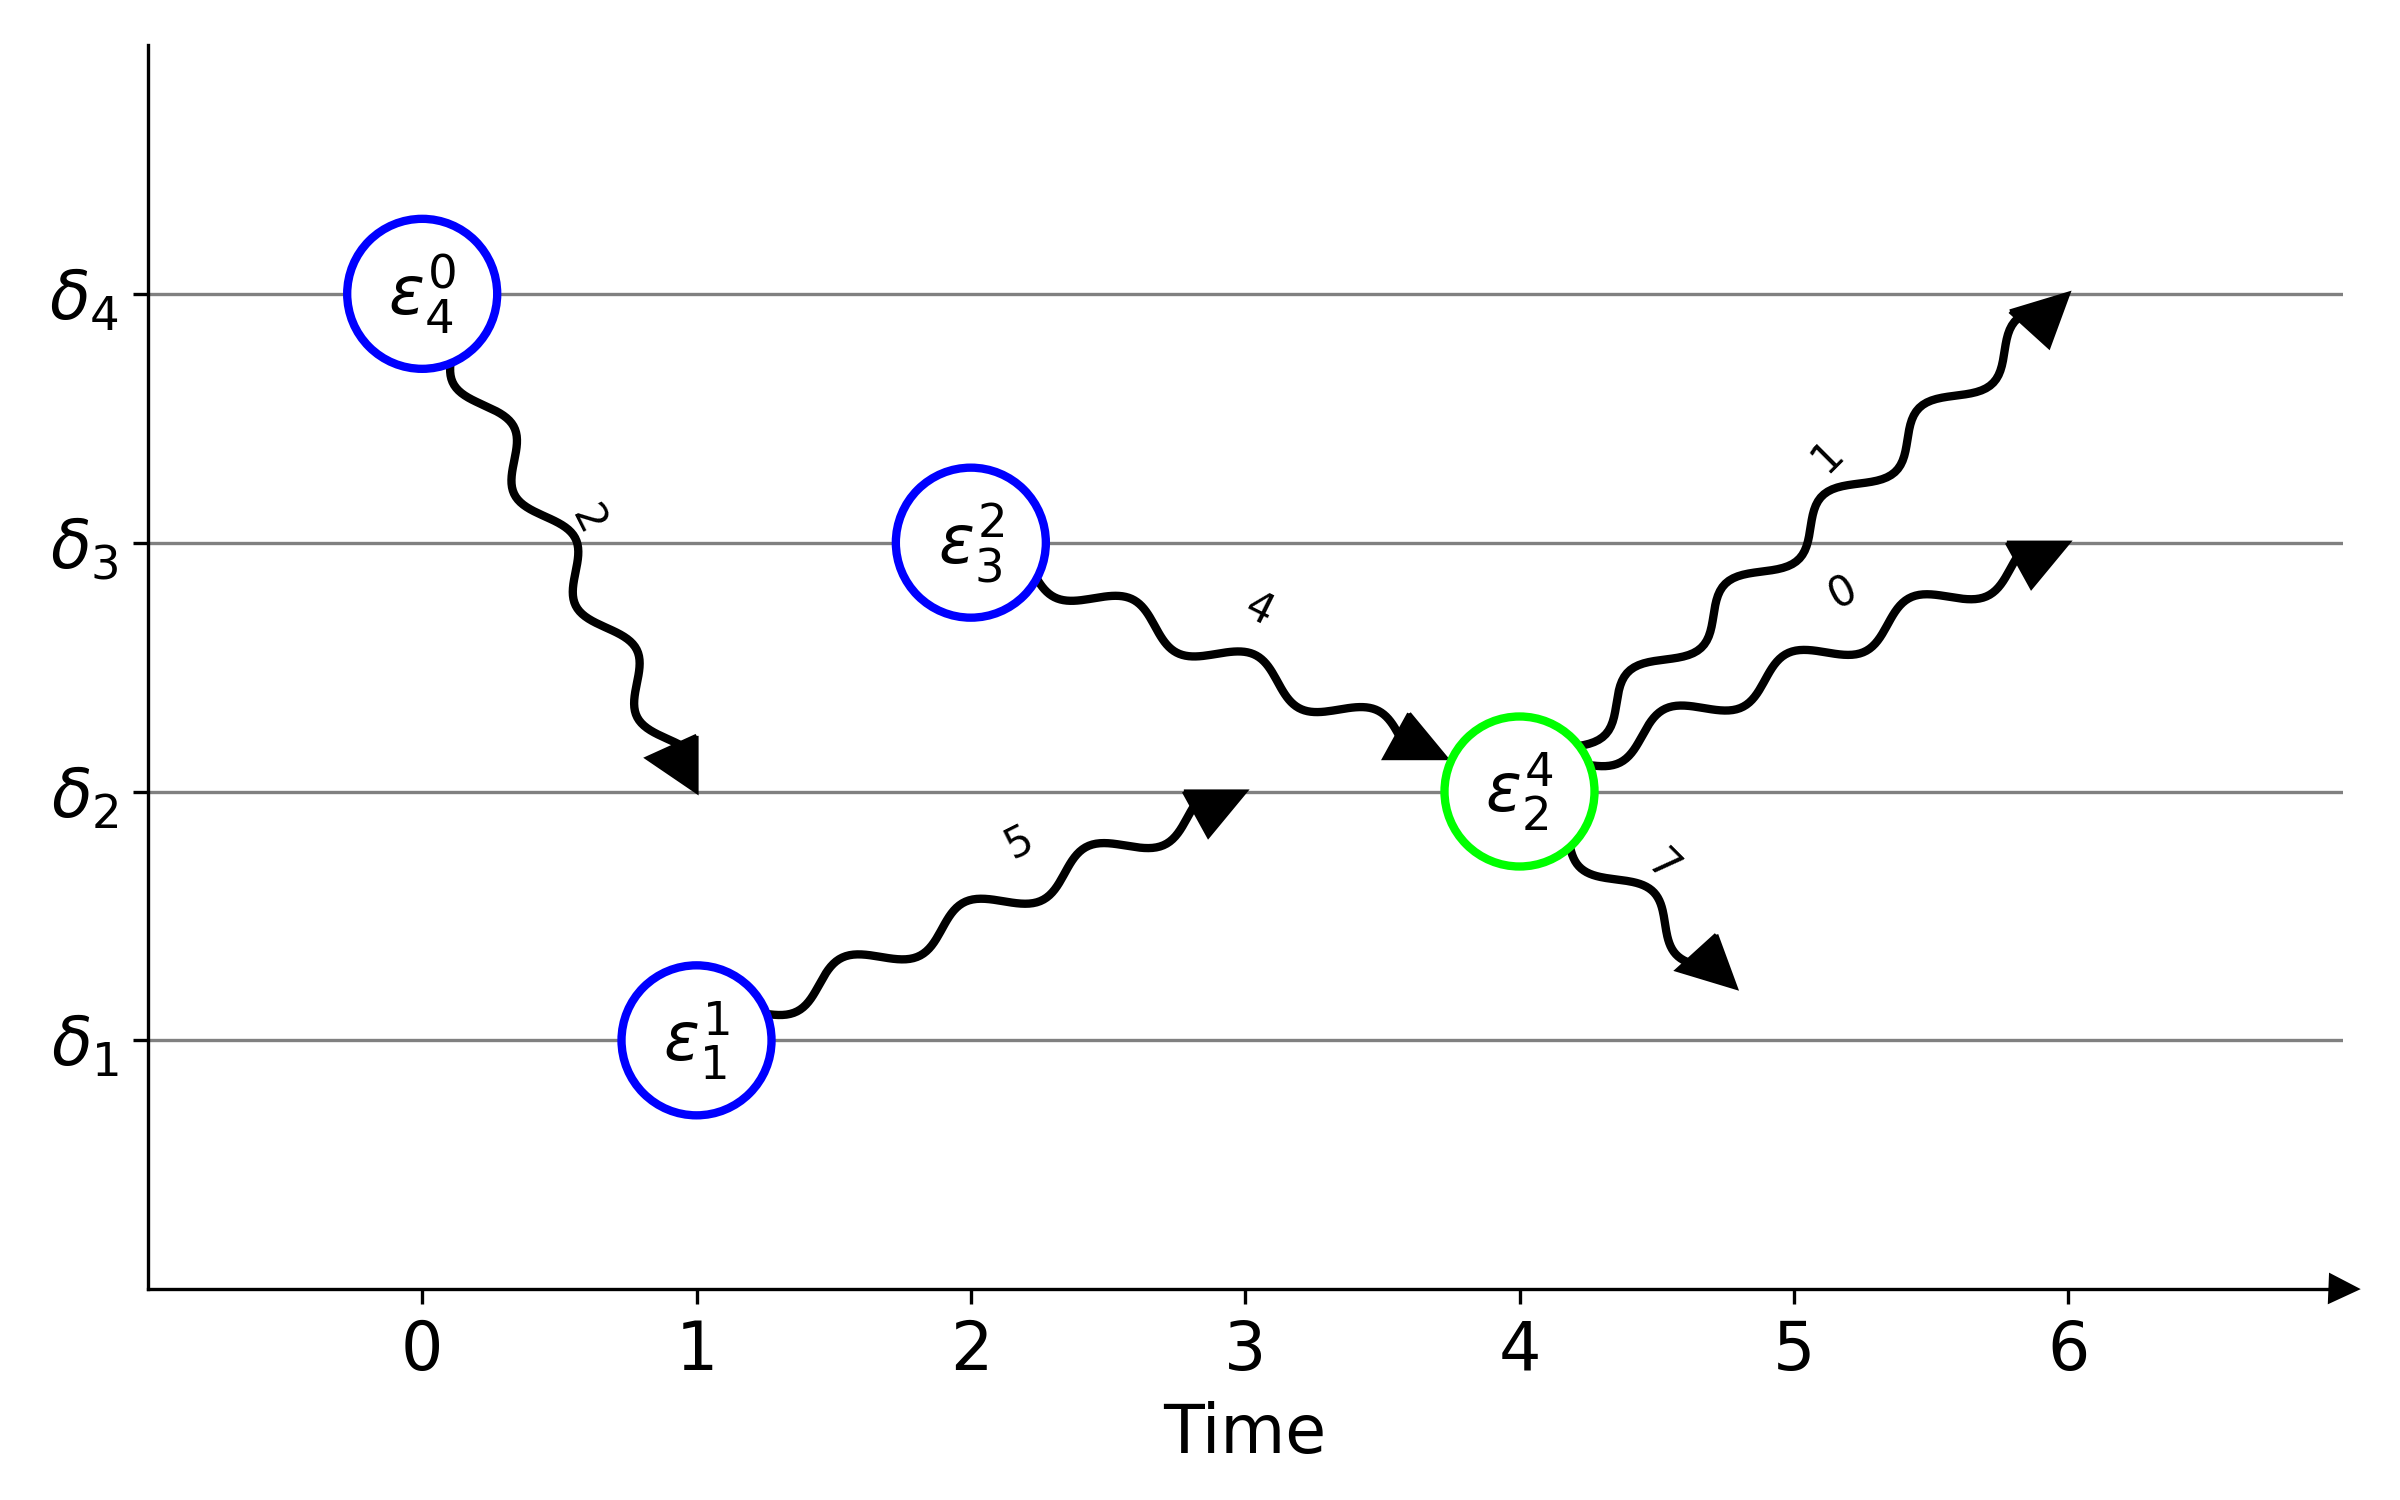
\includegraphics[width=.8\linewidth]{figures/nvalues-example.png}
    \caption{\ac{XC} system model, from the point of view of the wake-up event $\epsilon_2^4$ pictured in green.}
    \label{fig:xc-nvalues-exampke}
\end{figure}

\paragraph{Additional built-in operations} on nvalues are $self(\underline{\mathbf{w}} : \underline{A}) : A$ which returns the local value $\underline{\mathbf{w}}(\delta)$ for the self device $\delta$, and $updateSelf(\underline{\mathbf{w}} : \underline{A}, l : A) : \underline{A}$ which returns a new nvalue with the same content of $\underline{\mathbf{w}}$ but with the value for the self device replaced by $l$\cite{xc}.
%
Given the built-in function $uid$ that returns the device identifier of the self device, the following property holds: $self(\underline{\mathbf{w}}) = \underline{\mathbf{w}}(uid)$.
%
The complete syntax for \ac{XC} is available in the original paper\cite[p. 4]{xc}.

\subsection{The \texttt{exchange} primitive}

The following description is based on the original paper for \ac{XC}\cite{xc}.
%
The only communication primitive present in \ac{XC} is the function $$exchange(e_i, (\underline{\mathbf{n}}) \Rightarrow \mathbf{\return} e_r \mathbf{\send} e_s)$$ which is defined using syntactic sugar and translates to $$exchange(e_i, (\underline{\mathbf{n}}) \Rightarrow (e_r, e_s))$$
%
The evaluation of the primitive follows three steps:
\begin{enumerate}
    \item the device evaluates the expression $e_i$ to obtain the \textit{initial} local value $l_i$;
    \item $\underline{\mathbf{n}}$ is substituted with the nvalue $\underline{\mathbf{w}}$ of messages received from neighbors for this exchange, using $l_i$ as the default value for $\underline{\mathbf{w}}$, and the device evaluates the expression $e_r$ to the value $v_r$ to be returned;
    \item the device evaluates the expression $e_s$ to obtain a nvalue $\underline{\mathbf{w_s}}$ to be sent to neighbors such as $\delta'$, that will use their corresponding value $\underline{\mathbf{w_s}}(\delta')$ in their next execution round.
\end{enumerate}

As a shorthand, $$exchange(e_i, (\underline{\mathbf{n}}) \Rightarrow \mathbf{\return} e \mathbf{\send} e)$$ can be written as $$exchange(e_i, (\underline{\mathbf{n}}) \Rightarrow \mathbf{\retsend} e)$$ according to the \ac{XC} paper\cite{xc}.

Two examples of reusable functions written in \ac{XC} can be seen in \cref{lst:xc-program}.
%
There, $mux(cond, e_1, e_2)$ is a conditional expression that first evaluates $cond$, $e_1$, and $e_2$, and then returns the value of $e_1$ if $cond$ is true, or the value of $e_2$ otherwise.
%
\texttt{mux} is useful to avoid breaking the alignment of the network by using conditionals, as explained in \cref{chap:background->sec:xc->subsec:alignment}.
%
In the examples, $\underline{senseDist}$ is a network-based sensor that returns the nvalue containing the distances to neighbors, abstracting over the way the device obtains the measurements, with $Infinity$ as its default value used for all other devices.
%
\texttt{distanceEstimate} computes the minimum distance from a source using the distance sensor and the neighbors estimate $\underline{\mathbf{n}}$ of their minimum distance from the same source.
%
\texttt{distanceTo} computes the minimum distance from a source determined by a boolean expression, which is a \textit{gradient} with value $0$ in all devices where $src$ is true, and the minimum distance from the source in all other devices connected to a source device, or else $Infinity$.

\lstinputlisting[float,language=XC,label={lst:xc-program}, caption={Implementation of a network-wide gradient, called \texttt{distanceTo}, using the \ac{XC} language.}]{listings/xc-gradient-distance.xc}

\subsection{Alignment}\label{chap:background->sec:xc->subsec:alignment}

A program can execute multiple exchanges in a single round, and \ac{XC} ensures that messages are dispatched to corresponding exchange expressions, using the concept of \textit{alignment}.
%
The corresponding exchange expressions are those that are found in the same position in the \ac{AST} and the same stack frame, thus ensuring correct alignment in case of branches, function calls, and recursion\cite{xc}.
%
As a consequence, the evaluation of an aggregate program implicitly builds a tree representation, called \textit{value tree}, that all aligned devices, as well as the device itself in the next rounds, replicate and then exchange with each other.

Conditionals such as $if (cond) {e_1} else {e_2}$ interfere with alignment because only the \texttt{exchange} operations in the same position within the AST and stack frame align\cite{xc}.
%
As a consequence, \texttt{exchange} only aligns across devices that take the same branch of all the conditionals that are parent of the \texttt{exchange} operation in the AST.

Alignment controls the evaluation of sub-expressions, in particular the evaluation of expressions involving nvalues, because in such expressions only aligned neighbors are considered.
%
As a result, every \texttt{if} expression splits the network into two non-communicating sub-networks, each evaluating a different branch based on the condition\cite{xc}.
%
Isolated sub-networks in this regard are also called \textit{sub-domains}, or simply \textit{domains}.

\subsection{Formalization of XC}

\ac{XC} is formalized in the paper\cite{xc} in its syntax, operational semantics, and denotational semantics.
%
The language takes inspiration from \ac{ML}, and as such is a standard functional language with a classic Hindley-Milner type system, whose formalization makes \ac{XC} type sound and deterministic once extended with \textit{value-tree} typing and \textit{configuration} typing\cite{xc}.

\subsection{Implementing FC primitives with exchange}

With the implementation of \ac{FC} primitives and expressiveness using \ac{XC}, the \ac{XC} inherits all the results found in literature that hold for \ac{FC}, such as eventual recovery and stabilization after transient changes\cite{self-stabilisation-in-fc}, independence from the density of devices\cite{density-independence-in-fc}, real-time error tolerance and convergence\cite{real-time-error-tolerance-in-fc}, and the list continues\cite{xc}.
%
Additionally, \ac{XC} opens the possibilities for writing programs not expressible with \ac{FC}, thanks to the expressiveness of the \texttt{exchange} primitive which allows sending differentiated messages to neighbors.
%
In \ac{FC}, the concept of \textit{field}, also called \textit{neighboring value}, is defined as a neighbor-dependent value consisting of a map $\phi = \overline{\delta} \mapsto \overline{l}$ from neighbors to local values, which can be promoted to nvalue with any valid default value $l$.
%
This preserves the behavior of programs written in \ac{FC} but interpreted within \ac{XC}\cite{xc}.

\ac{FC} presents three main primitives to implement with \ac{XC}:
\begin{itemize}
    \item \texttt{nbr}, used to access the neighbors values\cite{from-dc-to-fc-and-ap};
    \item \texttt{rep}, used to compute a new value of an expression based on the result of the same expression in the previous round\cite{from-dc-to-fc-and-ap};
    \item \texttt{share}, used to efficiently access neighbors' values while computing a new value from the previous result with a single primitive\cite{share-operator}.
\end{itemize}

The \texttt{nbr} primitive can be implemented as: $$nbr(e: A): \underline{A} = exchange(e, (\underline{n}) \Rightarrow \return \underline{n} \send e)$$
%
The \texttt{rep} primitive can be implemented as: $$rep(e_i: A)\{(x) \Rightarrow e_n\}: A = exchange(e_i, (\underline{x}) => \retsend e_n[x := self(\underline{x})])$$
%
The \texttt{share} primitive can be implemented as: $$share(e_i: A)\{(\underline{x}) \Rightarrow e_n\}: A = self(exchange(e_i, (\underline{x}) => \retsend e_n))$$

\section{Scala 3}\label{chap:background->sec:scala3}

Scala 3 is the latest major release of the Scala language, a high-level programming language that combines object-oriented and functional programming paradigms.
%
Scala is a statically typed, general-purpose programming language designed to express common programming patterns in a concise, elegant, and type-safe way.
%
Scala 3 is compiled using the \textit{Dotty} compiler\footnote{\url{https://github.com/lampepfl/dotty}}, which is based on the \ac{DOT} calculus\cite{dot}, while Scala 2 is compiled using the \textit{scalac} compiler\footnote{\url{https://github.com/scala/scala}}.
%
This section provides an overview of the main features of Scala 3, which are relevant for the re-design of ScaFi, while also highlighting the differences between Scala 2 and Scala 3.

\subsection{General considerations on Scala 3}

Even though Scala 3 introduces breaking changes in the syntax from Scala 2, most of the code written in Scala 2 can be compiled with Dotty and is also binary compatible with Scala 2.
%
This possibility has been exploited by the Scala community to avoid reimplementing a new standard library for Scala 3, using the Scala 2 standard library instead, rewritten to be cross-compiled for both Scala 2 and Scala 3.

Originally, Scala 2 and Scala 3 compile to \ac{JVM} bytecode, but Scala 3 also supports the \ac{JS} and \textit{LLVM} backends, which are used to compile Scala code to JavaScript and native code, respectively, thanks to community-driven projects\footnote{Scala.js at \url{https://scala-js.org}}\footnote{Scala Native at \url{https://scala-native.org}}\cite{scala-js}.
%
The provided support for cross-platform distribution, together with the popularity of Scala for distributed systems development\cite{scala-popularity} and the flexibility of the upgraded language features for advanced internal \ac{DSL} design, makes Scala 3 a great choice for a new ScaFi implementation based on \ac{XC}.

\subsection{Values in Scala}

In Scala, every value has a type, following the type hierarchy explained in \cref{chap:background->sec:scala3->subsec:type-hierarchy}.
%
When declaring a new variable or field as a container of a value, the type can be explicitly declared, or it can be inferred by the compiler.
%
Every declaration of a variable or field must be preceded by the \texttt{val} keyword for an immutable value, or the \texttt{var} keyword for a mutable value.
%
Immutable values cannot be reassigned, while mutable values can be reassigned, but the type of the value cannot be changed.
%
\texttt{val} doesn't guarantee that the value itself is immutable, but only that the reference to the value cannot be changed.


\subsection{New control syntax and significant indentation}

Scala 3 introduced a new syntax for control expressions, as well as new rules that allow the indentation alone to replace the use of curly braces.
%
Both these changes are aimed at making the code more readable and concise, sometimes noticeably closer to the natural language.
%
For example, in \cref{lst:scala2-with-braces}, the \texttt{if} expression is written with the traditional syntax, while in \cref{lst:scala3-without-braces} the same expression is written using the new syntax.
%
The same is true of the \texttt{for} expression, the \texttt{while} loop, and the \texttt{match} expression.

\lstinputlisting[float,language=Scala,label={lst:scala2-with-braces}, caption={Examples of syntax using braces in Scala 2.}]{listings/scala2-with-braces.scala}
\lstinputlisting[float,language=Scala,label={lst:scala3-without-braces}, caption={Examples of syntax avoiding braces in Scala 3.}]{listings/scala3-without-braces.scala}

In cases where a code block consists of many lines that make it a bit hard to follow indentation, the new syntax can be combined with \texttt{end} statements, as shown in \cref{lst:scala3-with-end}.

\lstinputlisting[float,language=Scala,label={lst:scala3-with-end}, caption={Example of syntax using \texttt{end} statements in Scala 3.}]{listings/scala3-without-braces-with-end.scala}


\subsection{Traits and classes}

Traits are a powerful feature of Scala that replaces Java's interfaces and abstract classes and were first introduced as a mechanism to organize behavior into small, modular units\cite{traits}.
%
In Scala, traits can be used both to define interfaces and to provide partial implementations, composable and mixable into classes when a concrete implementation is needed.
%
With Scala 3, traits are now able to have parameters like classes do, enhancing their expressiveness.
%
Additionally, Scala 3 introduces new rules for instantiation of classes that allow to avoid the use of the \texttt{new} keyword, as shown in \cref{lst:scala3-without-braces}.
%
This feature is called \textit{universal apply methods} and is enabled by the generation of \texttt{apply} methods for classes done by the compiler when the user does not provide one.
%
This feature is enabled by a special role given to methods named \texttt{apply}, which in Scala can be invoked without the need to specify the method name.
%
When combined with companion objects, described in \cref{chap:background->sec:scala3->subsec:singleton-objects}, it is often possible to replace auxiliary constructor in classes with multiple \texttt{apply} methods in the companion object, which is a common pattern in Scala.
%
Anonymous classes make it possible to instantiate a trait or abstract class by providing a concrete implementation of abstract methods on the fly.
%
Just like in Java, traits, classes, and singleton objects can be nested and can access each other's private members.

If the definition of something depends on another from a different package, it is possible to use the \texttt{import} keyword to import the needed definitions.
%
\texttt{import} statements can be put at the beginning of a file, or inside a block, and can be used to import a single definition, a group of definitions, or all definitions from a package.
%
Additionally, Scala supports import aliases to avoid name clashes.
%
Since Scala 3, import aliases have a dedicated syntax, following the pattern \texttt{import A as B}, where \texttt{A} is the fully qualified original name and \texttt{B} is the alias.

An advanced example of trait usage can be found in \cref{lst:scala3-service-oriented-design}\footnote{\url{https://docs.scala-lang.org/scala3/book/domain-modeling-oop.html}}, which shows how to use traits in a service-oriented way, a design pattern that promotes the use of traits to define services and their dependencies and to compose services into a single class\cite{service-oriented-design}.
%
In the mentioned example, some advanced features of Scala are involved, such as abstract type members, nested traits, and \textit{self-type annotations}.
%
The \textit{self-type annotation} is a way to declare that a trait must be mixed into a class that extends another trait, and it is used to express dependencies between traits without using inheritance, allowing the composition of traits to be more flexible and less coupled, and delaying the choice of trait order to the class that mixes them.

\lstinputlisting[float,language=Scala,label={lst:scala3-service-oriented-design}, caption={Advanced example of usage of traits, know as service-oriented design. The code was taken from the Scala 3 book.}]{listings/scala3-service-oriented-design.scala}

\subsubsection{Object-oriented programming in Scala 3}

In Scala, classes, traits, enums, and objects can all have methods, defined using the \texttt{def} keyword, as seen in \cref{lst:scala3-without-braces}.
%
Abstract methods are methods that do not have a body and must be overridden by concrete subclasses, while concrete methods have a body and can be overridden by subclasses.
%
In Scala, a method with no arguments can be overridden by a field with the same name.
%
Many features of Scala allow methods to be used as operators, such as the infix notation, which allows to call methods with a single argument without using the dot or parentheses, as shown in \cref{lst:exchange-syntax}.
%
This feature provides great flexibility in the definition of custom operators, and the development of \ac{DSL}s.
%
Since Scala 3, the intent of the definition of custom operators is more explicit thanks to the \texttt{infix} keyword before \texttt{def}.

Even though method overloading is still possible, the Java generic type erasure rules apply in Scala too, and must be taken into account when defining overloaded methods.
%
In Scala, it is often possible to avoid method overloading by using default arguments, which are arguments that are automatically assigned a value if no value is provided by the caller, as shown in \cref{lst:scala3-extension-methods}.
%
Scala 3 improves the default way to handle method invocation ambiguities with method overloading with the \texttt{@targetName} annotation, which allows to specify a unique name of the method once compiled to \ac{JVM} bytecode.

Thanks to \textit{automatic eta expansion}, methods can be used in place of function values, and its implementation has been improved in Scala 3 to be almost completely seamless.

One of the most important features of Scala is the ability to define \textit{type members},
which are members of a class or trait that define types, and can be used as types in the same way as classes or traits, as shown in \cref{chap:background->sec:scala3->subsec:type-system}.
%
Abstract type members avoid Scala trait and class sources to grow in size both vertically and horizontally because they can often replace generic type parameters, with all the benefits of member inheritance, such as overriding and composition.

Type parameters as well as type members can be constrained with \textit{upper bounds} and \textit{lower bounds}, using the operators \texttt{<:} and \texttt{>:}, respectively, such as in \texttt{Type <: Supertype} and \texttt{Type >: Subtype}.
%
Generic types also support type variance control, which is used to specify how the subtyping relationship between two generic types is related to the subtyping relationship between their type arguments.
%
In Scala, the variance of a type parameter can be declared with the \texttt{+} and \texttt{-} symbols, which are used to declare a type parameter as covariant or contravariant, respectively, or else the type parameter is invariant by default.

\subsection{Algebraic Data Types}

The union of the object-oriented and the functional programming paradigms within Scala has always promoted the use of algebraic data types, a kind of composite type that resembles mathematical operations between types.
%
Examples of such types are \textit{sum types}, \textit{product types}, and \textit{intersection types}.
%
In Scala, these can be implemented using \textit{sealed traits}, \textit{case classes}, and inheritance, respectively, but from Scala 3 the syntax to define these types has been simplified and clarified, as shown in the following paragraphs.

\subsubsection{Sum types}

Since Scala 2, sum types were enabled by the \texttt{sealed} keyword on traits or abstract classes that prevent inheritance outside the file where the sum type is defined.
%
This way, it was possible to define a finite set of subtypes to check for in pattern matching.
%
Thanks to the possibility of defining a singleton instance with the keyword \texttt{object} that inherits from the sum type, sum types could also be used to implement enumerations.
%
Starting with Scala 3, the \texttt{enum} keyword has been introduced to simplify the syntax in both these use cases, as shown in \cref{lst:scala3-sum-types}.
%
Additionally, with Scala 3, the \texttt{|} operator can be used for sum type options in type definitions, for matching any pattern of a list in pattern matching, and for defining a discriminated union type of the form \texttt{A | B}.

\lstinputlisting[float,language=Scala,label={lst:scala3-sum-types}, caption={Example of sum types in Scala 3.}]{listings/scala3-enums.scala}

\subsubsection{Product types}

Since Scala 2, product types were enabled by the features provided by \textit{case classes}, which are Scala's implementation of the concept of \textit{records} in functional programming.
%
Case classes are classes equipped with compiler-generated methods for pattern matching, equality, copying, and printing.
%
In case classes, constructor parameters are public immutable fields by default, and the \texttt{copy} method can be used to create a new instance with some fields changed.
%
An example of a case class can be found in \cref{lst:scala3-sum-types}.

\subsubsection{Intersection types}

Since Scala 2, it was possible to define a type as the intersection of other types using the \texttt{with} keyword, which is also used for mixin composition.
%
Mixin composition is the practice of combining multiple traits into a class, resembling multiple inheritance but with the compromise of avoiding the diamond problem through linearization\cite{scala-patterns}.
%
Mixin composition is used in ScaFi to declare dependencies of programs, as shown in \cref{lst:using-libraries-in-scafi}.

Starting with Scala 3, the \texttt{with} keyword is deprecated for type definitions, such as in method arguments, in favor of the \texttt{\&} operator, which is also used for pattern matching, as in \cref{lst:lst:distance-to}, in the \texttt{distanceTo} signature.
%
The \texttt{with} keyword is still used for mixin composition in the definition of traits and classes.


\subsection{Singleton objects} \label{chap:background->sec:scala3->subsec:singleton-objects}

In Scala, the \texttt{object} keyword is used to define a singleton object, which is a class that has only one instance.
%
Singleton objects replace Java's static methods and fields and can be used to define utility methods and constants, as well as to implement the \textit{companion object} pattern, which is a design pattern that promotes the use of a singleton object to hold methods and fields that are not specific to any instance of a class but are still related to the class itself.
%
A class with a companion object can access the private members of the companion object, and vice versa, provided that they have the same name and are defined in the same file.
%
Singleton objects can be also used to implement traits to create modules, such as factories for collections.
%
An example of a singleton object used as a companion of a class can be found in \cref{lst:scala3-singleton-object}.

\lstinputlisting[float,language=Scala,label={lst:scala3-singleton-object}, caption={Example of a singleton object in Scala 3.}]{listings/scala3-singleton-object.scala}


\subsection{Functional programming with Scala 3} \label{chap:background->sec:scala3->subsec:functional-programming}

Scala offers many features typical of \ac{FP} languages, such as \textit{lambdas}, higher-order functions, \textit{currying}, algebraic data types, and a standard library of immutable collections.
%
Lambdas, also known as anonymous functions, can be passed as an argument or returned as a result just like any other value.
%
A function that accepts or returns another function is called a \textit{higher-order function}.
%
In Scala, lambdas are defined using the \texttt{=>} operator, which is also used to define function types such as \texttt{A => B}, where \texttt{A} is the input type and \texttt{B} is the output type.
%
Sometimes it is possible to write lambdas with a more concise syntax, using the \texttt{\_} placeholder for the input argument, as shown in \cref{lst:foldhood-library-usage}.

Starting with Scala 3, function types support new varieties of functions:
\begin{itemize}
    \item \textit{dependent function types}, which are function types where the result type can depend on the function's parameters, such as type members (an example can be found in \cref{lst:distance-to});
    \item \textit{polymorphic function types}, which are function types that accept type parameters, explained in \cref{chap:background->sec:scala3->subsec:type-system};
    \item \textit{context function types}, which are function types that accept only context parameters, explained in \cref{chap:background->sec:scala3->subsec:contextual-abstractions}.
\end{itemize}

Following the principles of \ac{FP}, domain models should be immutable and deprived of behavior, and behavior should be defined in terms of pure functions, implemented in modules as extension methods, which are methods that can be added to existing types without modifying their source code.
%
Starting with Scala 3, extension methods have obtained a dedicated syntax, that avoids the cumbersome use of implicit classes, as shown in \cref{lst:scala3-extension-methods}.
%
Some additional attention is needed when extension method names overlap with class methods, because the compiler will always prioritize the class method, and the extension method will be shadowed.
%
In those cases it is always possible to invoke the extension explicitly from the instance that provides it, passing the extended instance as the first argument.

\lstinputlisting[float,language=Scala,label={lst:scala3-extension-methods}, caption={Example of extension methods usage in Scala 3.}]{listings/scala3-extension-methods.scala}

\paragraph{Currying} is the process of transforming a function that takes multiple arguments into a sequence of functions, each taking a subset of the arguments, thus simplifying the function's usage with partial applications.
%
An example of currying and partial application of a function can be found in \cref{lst:scala3-currying}.

\lstinputlisting[float,language=Scala,label={lst:scala3-currying}, caption={Example of currying and partial application in Scala 3.}]{listings/scala3-currying.scala}


\subsection{Contextual Abstractions} \label{chap:background->sec:scala3->subsec:contextual-abstractions}

In Scala, contextual abstractions are a set of features coming from the core idea of \textit{term inference}, which is the ability of the compiler to synthesize a \quotes{canonical} term for a given type.
%
Examples of features enabled by term inference are \textit{extension methods}, \textit{type classes}, \textit{context parameters}, \textit{context bounds}, and many more.
%
In Scala 2, almost every feature of contextual abstractions was implemented using the \texttt{implicit} keyword, whereas with Scala 3 contextual abstractions have been redesigned to be more explicit on the intent of their usage, with the introduction of new ad-hoc keywords for each use case: \texttt{given}, \texttt{using}, and \texttt{extension}.
%
The \texttt{given} keyword is used to define a \textit{given instance}, which is a value that can be used as a \textit{context parameter} in a method or constructor.
%
The \texttt{using} keyword is used to specify a \textit{context parameter}, also called implicit parameter in Scala 2, which is a parameter that is used to require a \textit{given instance} for a method or constructor.
%
The \texttt{extension} keyword is used to define an \textit{extension method}, which is a method that can be added to existing types without modifying their source code, as explained in \cref{chap:background->sec:scala3->subsec:functional-programming}.
%
If not passed explicitly, the compiler searches for \textit{given instances} to satisfy \textit{context parameters} performing \textit{term inference}.
%
Starting with Scala 3, context parameters can be anonymous, and given instances can be abstract.
%
To retrieve the value of an anonymous context parameter of type \texttt{T} Scala 3 provides the \texttt{summon[T]: T} method, that replaces Scala 2's \texttt{implicitly[T]} method.

\textit{Context bounds} in the form \texttt{T: Type} are syntactic sugar for context parameters with a more concise syntax, that gets desugared by the compiler to a context parameter of type \texttt{Type[T]}, as shown in .
%
An abstract class like \texttt{Type[T]} meant to be used to add behavior to any closed data type without sub-typing is called a \textit{type class}.
TODO add examples of context bounds desugar

Given instances can be imported and exported using the \texttt{import} and \texttt{export} keywords, but starting with Scala 3, \textit{given imports} and \textit{given exports} require the \texttt{given} keyword, even in the cases where a wildcard is used, making more clear where givens in the current scope are coming from.
%
Concrete given instances can be anonymous, in which case the compiler synthesizes a name for them.
%
This feature is useful to avoid polluting the namespace with names that are not meant to be used directly by the user, because often given instances are imported by their type instead of by their name.

Starting with Scala 3, implicit conversions are defined by providing given instances of the type \texttt{Conversion[From, To]}, and must be enabled with a compiler flag to avoid warnings when conversion is silently applied before passing an argument to a function call.
%
By default, the scala compiler provides implicit conversions for primitive types, such as \texttt{Int} to \texttt{Long}.


\subsection{The Scala 3 type system} \label{chap:background->sec:scala3->subsec:type-system}

Scala, as a statically typed language, has all the benefits of static typing, such as early error detection, better performance, and better tooling support, while also leveraging its features to feel like a dynamically typed language, such as type inference, type parameters, and type members.
%
Scala has always supported a strong type inference system, powered by a variant of the Hindley-Milner type system with support for subtyping, as well as generics and type bounds like in Java.
%
Additionally, Scala adds many type system features that are not present in Java, such as \textit{type variance}, \textit{type aliases}, \textit{type members}, \textit{covariant and contravariant overriding}, \textit{higher-kinded types}
%
Furthermore, starting with Scala 3, the type system features \textit{opaque type aliases}, \textit{structural types}, \textit{dependent function types}, improved \textit{type lambdas}, \textit{polymorphic function types}, \textit{context function types}, and \textit{match types}.

In the next paragraphs, the most relevant features of the Scala 3 type system are explained.

\paragraph{Type variance} allows to specify how the subtyping relationship between two generic types is related to the subtyping relationship between their type arguments.
%
In Scala, the variance of a type parameter can be declared with the \texttt{+} and \texttt{-} symbols, which are used to declare a type parameter as covariant or contravariant, respectively, or else the type parameter is invariant by default.

TODO insert example as listing

\paragraph{Type aliases} are used to define a new name for an existing type, and are often used to provide more descriptive names for types, or to shorten long type names.
%
Type aliases can be parameterized and can be recursive.
%
Their syntax is the same for defining type members, using the \texttt{type} keyword, as shown in
%
Opaque type aliases are a new feature of Scala 3 that allows defining a type alias that is not interchangeable with its underlying type, hiding it from consumers.

TODO insert example as listing

\paragraph{Covariant and contravariant overrides} allow to override a method defined in a superclass with a method that has a more specific return type or a more general parameter type, respectively.

TODO insert example as listing

\paragraph{Higher-kinded types} allow to define types and methods that work with generic types regardless of the actual type arguments, only requiring a fixed arity of type parameters.
%
Scala types are partitioned into kinds, based on the top type of which it is a subtype, such as \texttt{Any}, \texttt{[+X] =>> Any}, \texttt{[X, +Y] =>> Any}.
%
Higher-kinded types are types whose kind counts more than zero type arrows, such as \texttt{List} of kind \texttt{[+X] =>> Any}, \texttt{Option} of kind \texttt{[+X] =>> Any}, and \texttt{Map} of kind \texttt{[X, +Y] =>> Any}, but potentially even a type whose kind is \texttt{[X] => [Y] => Any}, such as a type class for a type constructor.
%
Scala 3 adds support for \textit{kind polymorphism}, which allows to define type parameters that accept types of any kind, through the special syntax \texttt{T <: AnyKind}.

TODO insert example as listing

\paragraph{Type lambdas} are simply anonymous type constructors, that starting from Scala 3 have a new syntax that allows to define them more concisely, using the type operator \texttt{=>>}.
%
For instance, \texttt{[X, Y] =>> Map[Y, X]} is a binary type constructor that maps arguments \texttt{X} and \texttt{Y} to the type \texttt{Map[Y, X]}.

\paragraph{Context functions} are functions that accept only context parameters as input. Starting with Scala 3, context functions can be treated as values thanks to context function types, which can be distinguished from normal function types by the presence of the \texttt{?=>} operator in place of the \texttt{=>} operator.

\paragraph{Match types} are conditional type aliases that allow the definition of a type as the result of a pattern match on a type, available since Scala 3.
%
An example of match types can be found in \cref{lst:scala3-match-types}.

\lstinputlisting[float,language=Scala,label={lst:scala3-match-types}, caption={Example of match types in Scala 3.}]{listings/scala3-match-type.scala}


\subsection{Explicit nulls and the Scala 3 type hierarchy} \label{chap:background->sec:scala3->subsec:type-hierarchy} \label{chap:background->sec:scala3->subsec:explicit-nulls}

The Dotty compiler allows to enable some experimental features that change the language in various ways.
%
Two examples of experimental features relevant to \this are \textit{explicit nulls} and the \textit{multiversal equality}.

Explicit nulls are enabled by the \quotes{\texttt{-Yexplicit-nulls}}, and the effect of this flag is to change the type hierarchy of Scala to make reference types non-nullable.
%
With explicit nulls disabled, the type system looks like the one in Java, pictured in \cref{fig:scala-hierarchy-with-explicit-nulls-disabled}, whereas with explicit nulls enabled, the type system looks more like the one in Kotlin, where null safety is part of the language, pictured in \cref{fig:scala-hierarchy-with-explicit-nulls-enabled}.
%
To define a nullable value with the option enable, sum types can be used, such as in \texttt{Type | Null}.
%
Scala 3 provides an extension method \texttt{.nn} to convert a nullable value to a non-nullable value, through casting, resulting in \textit{NullPointerException} if the value was \texttt{null} at runtime.

\begin{figure}
    \centering
    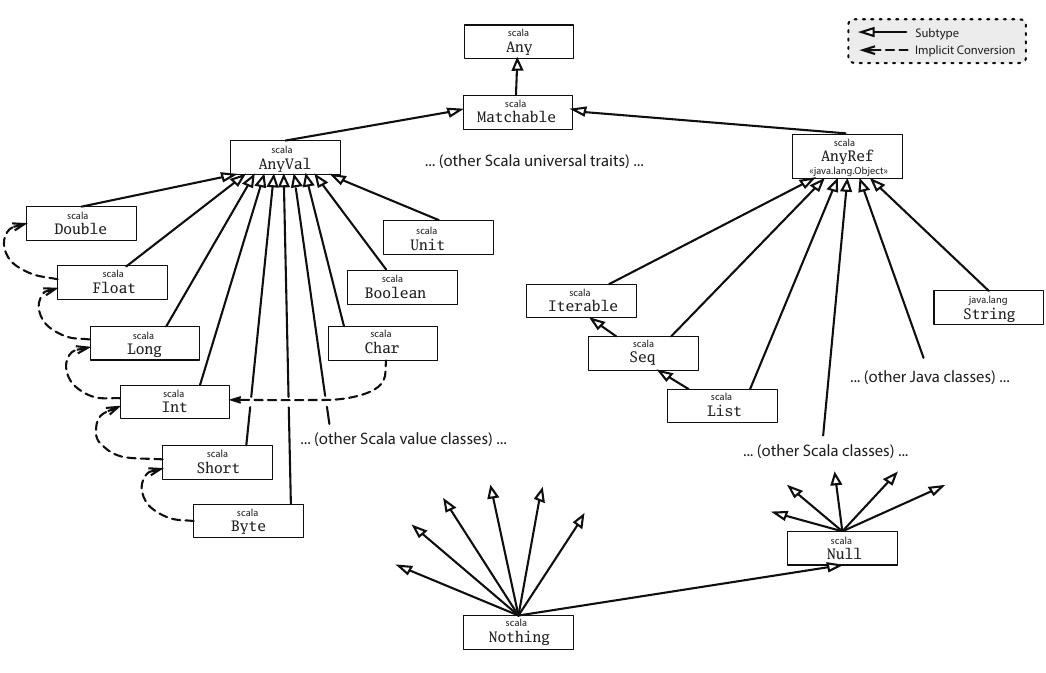
\includegraphics[width=.8\linewidth]{figures/scalaHierarchyWithMatchable.png}
    \caption{Scala type hierarchy with explicit nulls disabled.}
    \label{fig:scala-hierarchy-with-explicit-nulls-disabled}
\end{figure}

\begin{figure}
    \centering
    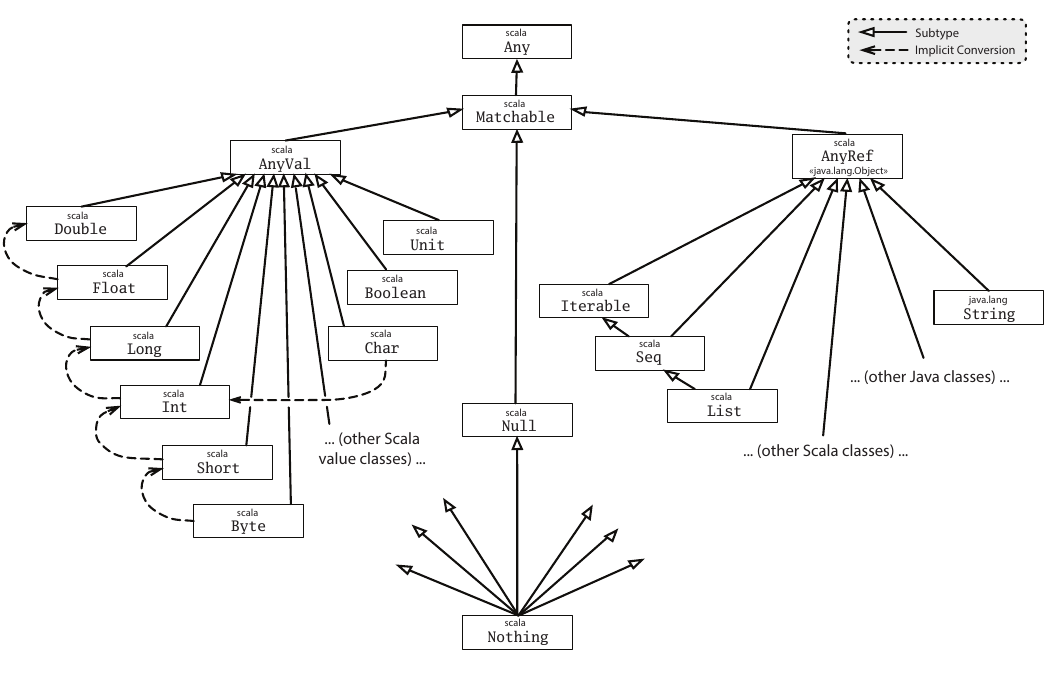
\includegraphics[width=.8\linewidth]{figures/scalaHierarchyWithMatchableAndSafeNull.png}
    \caption{Scala type hierarchy with explicit nulls enabled.}
    \label{fig:scala-hierarchy-with-explicit-nulls-enabled}
\end{figure}


\subsection{Multiversal Equality} \label{chap:background->sec:scala3->subsec:multiversal-equality}

Using context parameters of type \texttt{CanEqual[X, Y]}, the Scala 3 compiler with the \quotes{\texttt{-language:strictEquality}} flag enabled forbids universal equality, that allowed comparing any two values of any type, and replaces it with multiversal equality, which allows comparing any two values of any type, but only if the compiler can prove that the types are related by a \texttt{CanEqual} instance.
%
Implementing \texttt{CanEqual[X, Y]} instances can be automated with \textit{type class derivation}, a feature of Scala 3 that allows the compiler to synthesize given instances following rules defined by the user, often based on compositions of algebraic data types.


% ! TeX root = ../thesis-main.tex
%----------------------------------------------------------------------------------------
\chapter{Analysis}
\label{chap:analysis}
%----------------------------------------------------------------------------------------
This chapter defines the scope, requirements, and use cases of \this, as well as their analysis and prioritization.

\section{Requirement analysis} \label{chap:analysis->sec:requirement-analysis}

Since the very beginning, \this aimed to redesign ScaFi using Scala 3 to improve the quality of the code, including but not limited to readability, maintainability, and reusability.
%
This time, using the \ac{XC} as the theoretical foundation, through which the \ac{FC} constructs could be implemented.

The project started interviewing the stakeholders, which are the developers and researchers who use ScaFi, to understand their needs and expectations.

The \textit{key users} identified for the library are:
\begin{itemize}
    \item \textit{End users}, that is, the developers who will use the library to implement their aggregate programs;
    \item \textit{Library developers}, who will extend the library with new features, constructs, and syntax;
    \item \textit{Researchers}, who will experiment with the calculus foundations but would benefit from reusing existing libraries.
\end{itemize}

During the interviews, both functional and technical requirements emerged and were collected and given priorities based on further discussions and feedback from the stakeholders.

\paragraph{Functional requirements} are the features that the library must provide to the users. The following are the most relevant functional requirements identified:
\begin{enumerate}[label=\textbf{F.\arabic*}]
    \item Redesign and implement a new \ac{API} for the \texttt{core} package\cref{chap:analysis->sec:scafi-analysis};
    \item Redesign and implement the \texttt{tests} package with acceptance tests, easy to read and understand, and that can be used as examples;
    \item Use the \ac{XC} as the foundation of the (default) implementation of constructs, while still providing a \ac{FC} based API;
    \item Develop an \textit{Alchemist incarnation}\footnote{\url{https://github.com/AlchemistSimulator/Alchemist}}\cite{alchemist}, enabling \this programs to run on the well-tested and widely used Alchemist simulator;
    \item Develop a minimal, pure Scala 3 simulator to run tests and examples without the need for external dependencies;
    \item Provide a new API for the \texttt{core} package that allows developers to import arbitrary ScaFi libraries and constructs into their programs without conflicts, in a seamless way;
    \item Prefer keeping the original, abbreviated names for core constructs like \texttt{nbr} and \texttt{rep}, now that they are widely adopted and recognized by the community;
    \item Experiment with Scala 3 to achieve new, compile time features for ScaFi that can improve the quality of the code and the user experience.
\end{enumerate}

\paragraph{Technical requirements} are the constraints and guidelines that the library must follow to ensure the quality of the code and the user experience.
\begin{enumerate}[label=\textbf{T.\arabic*}]
    \item Use Scala 3 as the host language;
    \item Enable quality options on the Scala 3 compiler such as explicit nulls (\cref{chap:background->sec:scala3->subsec:explicit-nulls}) and multiversal equality (\cref{chap:background->sec:scala3->subsec:multiversal-equality});
    \item Use \ac{SBT} as build system;
    \item Cross-build the project for \textit{scala-js}\footnote{\url{https://www.scala-js.org}};
    \item Cross-build the project for \textit{scala-native}\footnote{\url{https://scala-native.org}};
    \item Lint the code with \textit{scalafix}\footnote{\url{https://scalacenter.github.io/scalafix}} and/or \textit{scalafmt}\footnote{\url{https://scalameta.org/scalafmt}};
    \item Avoid using third-party libraries for the \texttt{core} package dependencies.
\end{enumerate}

Then, the requirements were discussed and prioritized, following the \ac{MoSCoW} method,
resulting in the table in \cref{tab:requirements-prioritization}.

\begin{table}[ht]
\centering
\caption{Requirements prioritization.}
\label{tab:requirements-prioritization}
\begin{tabular}{|>{\hspace{0pt}}m{0.362\linewidth}|>{\hspace{0pt}}m{0.277\linewidth}|>{\hspace{0pt}}m{0.238\linewidth}|} 
    \hline
    \textbf{Requirement} & \textbf{MoSCoW} & \textbf{Priority}  \\ 
    \hline
    F.1          & must   & high      \\ 
    \hline
    F.2          & must   & high      \\ 
    \hline
    F.3          & must   & high      \\ 
    \hline
    F.4          & could  & low       \\ 
    \hline
    F.5          & must   & high      \\ 
    \hline
    F.6          & should & average   \\ 
    \hline
    F.7          & should & average   \\ 
    \hline
    F.8          & won't  & low       \\ 
    \hline
    T.1          & must   & high      \\ 
    \hline
    T.2          & should & high      \\ 
    \hline
    T.3          & must   & high      \\ 
    \hline
    T.4          & could  & low       \\ 
    \hline
    T.5          & could  & low       \\ 
    \hline
    T.6          & should & low       \\ 
    \hline
    T.7          & should & average   \\
    \hline
\end{tabular}
\end{table}

Finally, before starting with the design of the solution, given that the project is a redesign of an existing library, the requirements were compared with the existing ScaFi library to identify the differences and similarities.



\section{ScaFi} \label{chap:analysis->sec:scafi-analysis}

The ScaFi repository\footnote{\url{https://github.com/scafi/scafi}} is organized in modules as pictured in \cref{fig:scafi-project-org}.
%
For most of the use cases, only a small subset of the modules should be imported.
%
The \this project is scoped around redesigning and implementing mainly the \texttt{core} package, implicitly including \texttt{commons}, and then the \texttt{simulator} and \texttt{tests} packages, albeit with a minimal version of the simulator in pure Scala 3.
%
The rest of the modules, providing various \ac{GUI} implementations, demos, as well as integration with \textit{Akka}\footnote{\url{https://akka.io}} for actual deployment of real-world aggregate applications, are out of the scope of \this, and are addressed in \cref{chap:conclusion-and-future-work}.

\begin{figure}
    \centering
    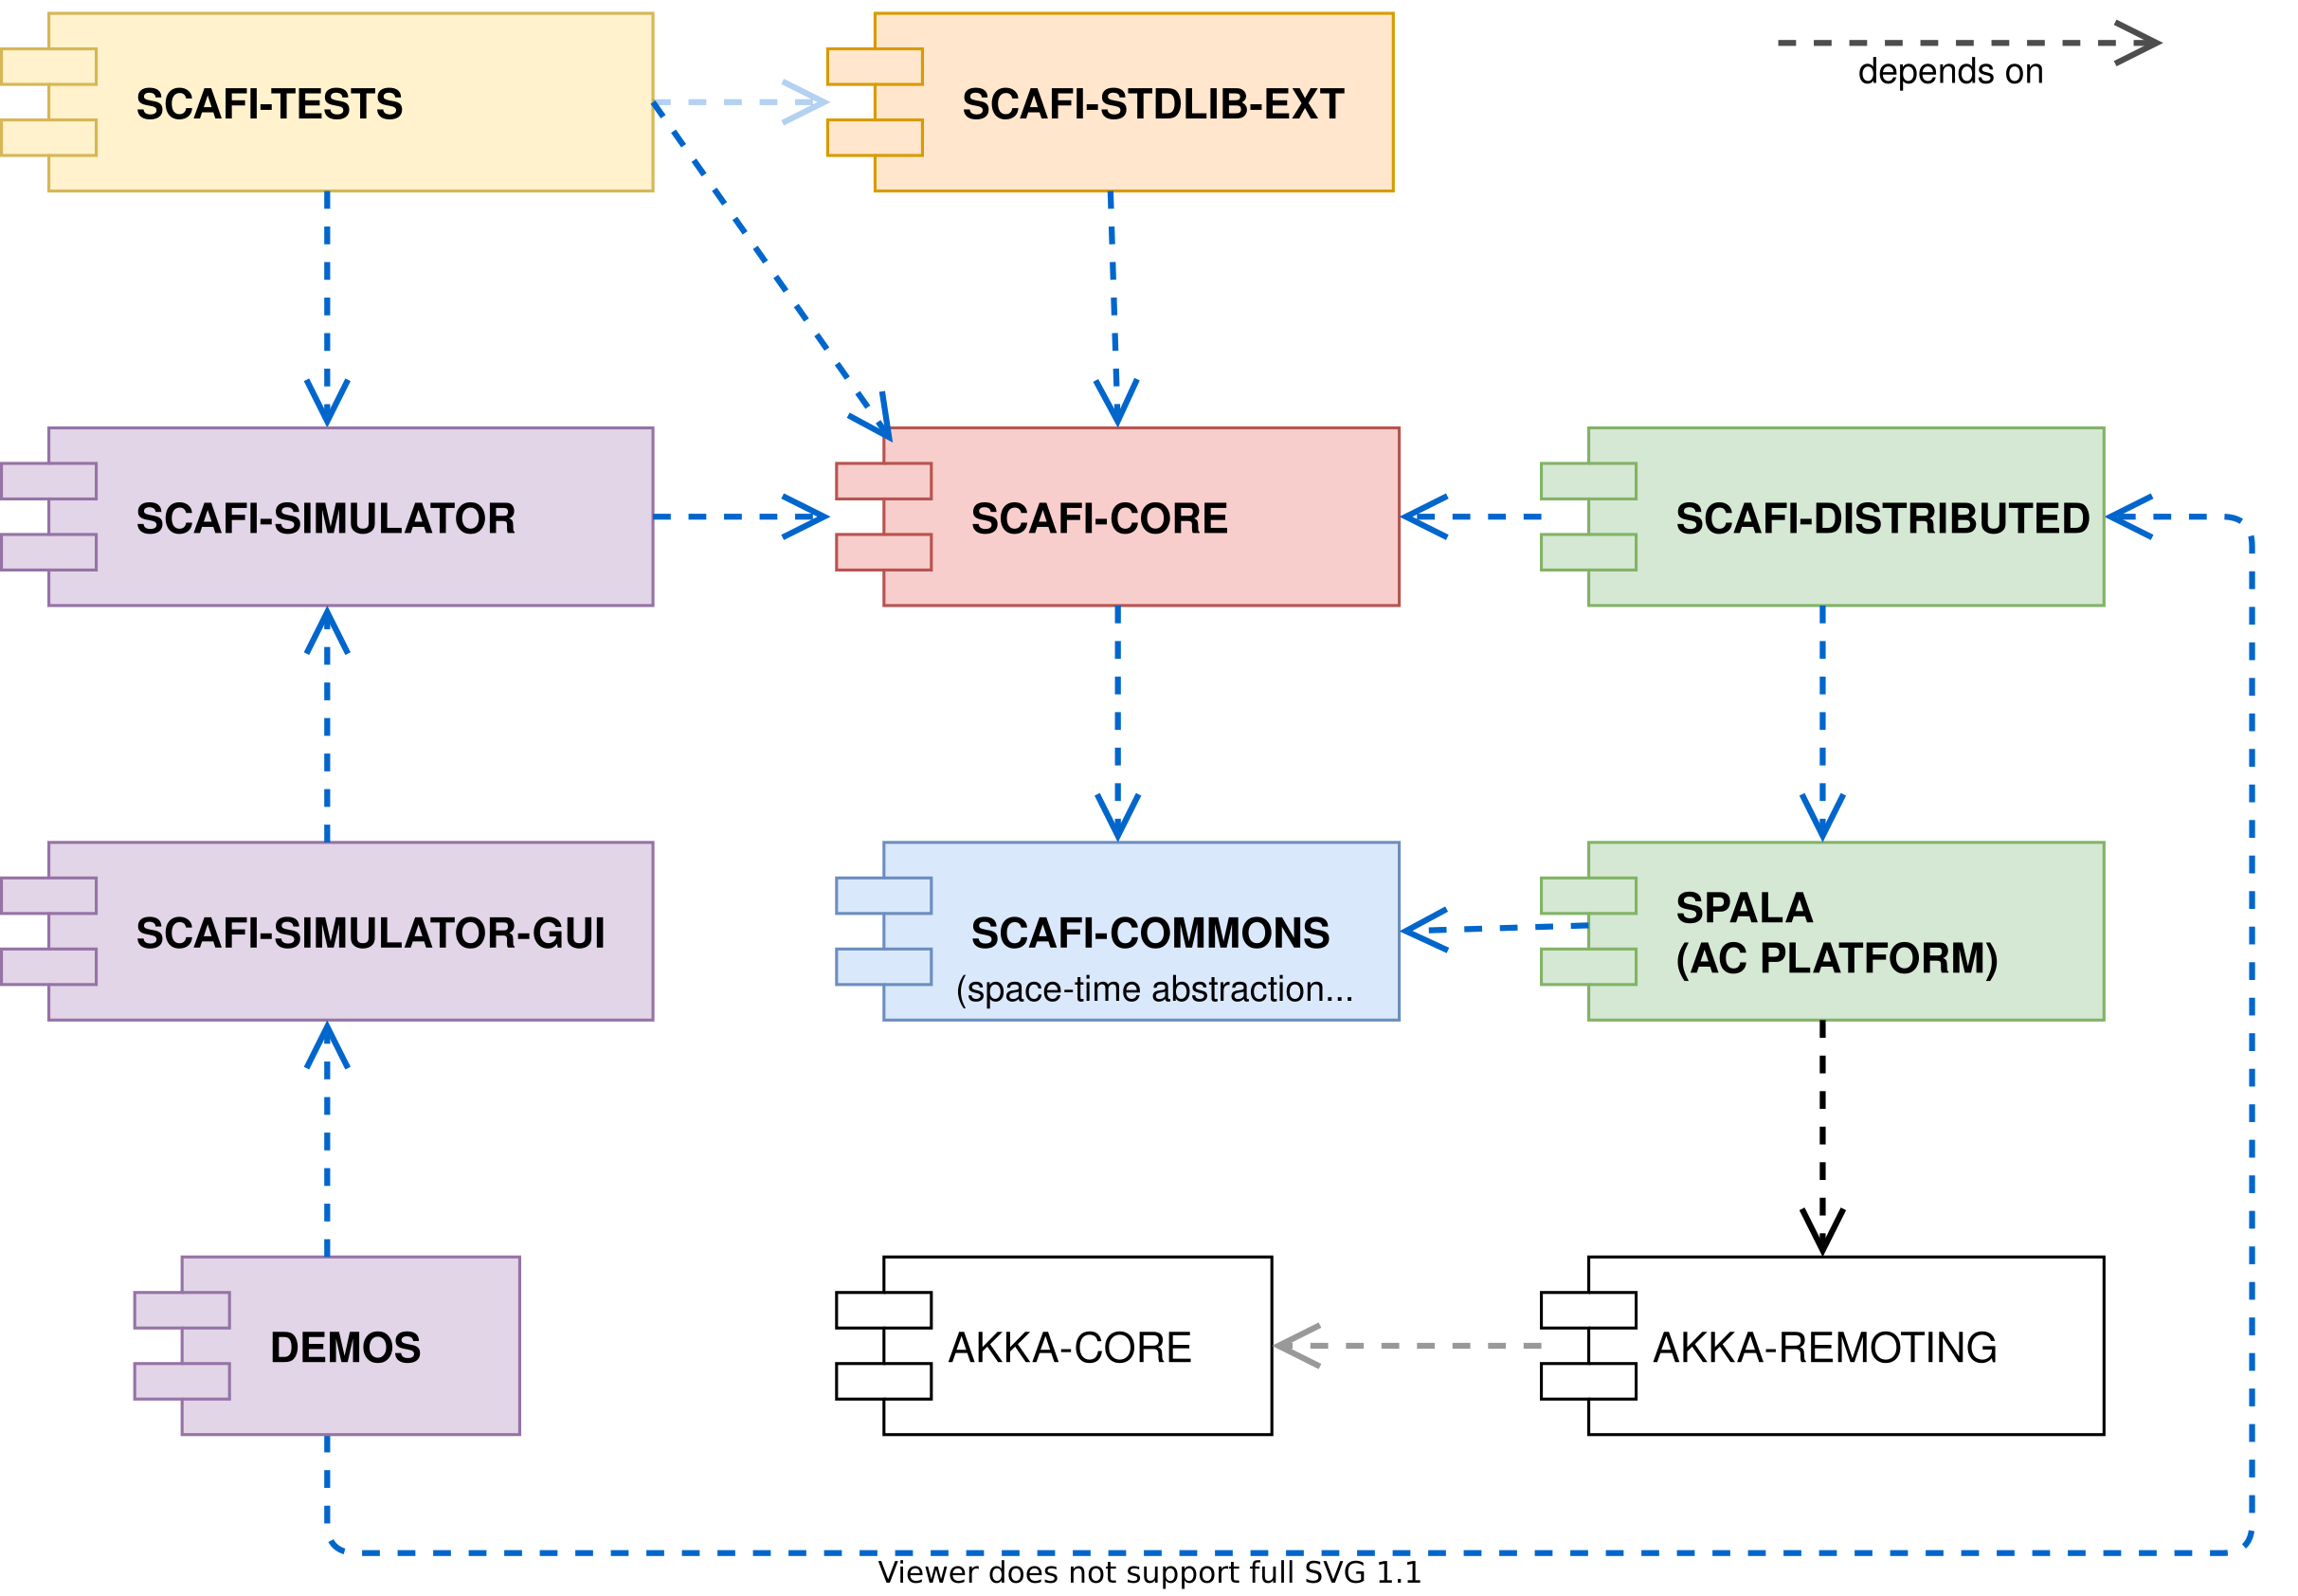
\includegraphics[width=.8\linewidth]{figures/scafi-project-org.drawio.png}
    \caption{ScaFi project organization.}
    \label{fig:scafi-project-org}
\end{figure}


To use a library component in ScaFi, the user must mix in the library trait with the \texttt{AggregateProgram} base class, as shown in \cref{lst:using-libraries-in-scafi}.

\lstinputlisting[float, language=Scala, caption={Using a library component in ScaFi.}, label={lst:using-libraries-in-scafi}]{listings/scafi-using-libraries.scala}

TODO go on


% ! TeX root = ../thesis-main.tex
%----------------------------------------------------------------------------------------
\chapter{Design}
\label{chap:design}
%----------------------------------------------------------------------------------------
The design of \this has been divided into three main phases.
%
In the first part, four design prototypes have been developed in order to choose the best user experience for three key users, the \textit{program developer}, the \textit{library developer}, and finally \textit{a new foundation researcher}, which represents a novelty in the use cases of an aggregate programming library.
%
More on that can be found in \cref{chap:design->sec:dsl}

In the second part, the final version of the \ac{DSL} has been designed, taking the best features from the prototypes and integrating them into a new core \ac{DSL} for \this.

In the third and final part, the design process concerned the simulator and the testing suites, also designed to scale with future extensions of the \ac{DSL}, as well as to be used as a reference for the \textit{program developer} and the \textit{library developer}, and to be as readable and understandable as possible, effectively working as acceptance tests.

TODO link design process to requirements from the analysis chapter

\section{Designing a scalable internal Domain Specific Language} \label{chap:design->sec:dsl}

The process of designing a new core \ac{DSL} for \this has been carried out through rapid prototyping of four competing designs of different \acp{DSL}, each coming with a set of advantages and disadvantages, highlighted using code snippets for every key user.
%
Prototipation has been necessary to explore the design space and to understand the trade-offs between different design choices, as well as to test in practice the interactions of different combinations of language features.
%
For each of the four prototypes, a brief description of the design choices and the programming experience is provided, followed by the final design described in \cref{chap:design->sec:final-dsl}.
%
Each prototype is named after the Scala 3 feature it's mainly based on, and each aims to separate the definition of the syntax from the definition of the semantics, and separate the definition of the semantics from the actual implementation.
%
This way, more than one semantic can be defined for the same syntax, and more than one implementation can be defined for the same semantic, allowing for more flexible customization and composition.
%
For the scope of \this, \ac{XC}\cite{xc} is the only semantics considered for implementation, but the design should be flexible enough to allow for future \quotes{calculi} to be implemented as alternative foundations.
%
In practice, there is a very subtle difference between the semantics and the syntax of the same formal calculus.
%
In the case of \ac{XC}, the syntax and the semantics both consist of two methods, \texttt{branch} and \texttt{exchange}.
%
The difference lies in the role of the two methods in the two contexts: in the syntax, they are constructs that the programmer uses to write programs, and should be treated as an \ac{API} at all effects, while in the semantics, they are constructs that the programmer uses to implement all the supported syntaxes \ac{API}, meaning they are not part of an \ac{API} used by aggregate programs and are focused on being as complete and simple to implement as possible.
%
For instance, the \texttt{exchange} method of the \texttt{ExchangeCalculusSyntax} trait is focused on its usage experience, attempting to mimick the syntax provided in the paper, meanwhile the \texttt{xcexchange} method of the \texttt{ExchangeCalculusSemantics} has \texttt{protected} visibility and its signature provides only the most complete and expressive version of the \texttt{exchange} primitive presented in the paper\cite{xc}.

Each of the four prototypes retains the separation between syntax definitions, semantic definitions, syntax support declaration, and semantics implementations, and considers the programmer experience of all the three key users.
%
For brevity, only the most relevant advantages and disadvantages are highlighted, and the full code of the prototypes is available in the project repository git history, under the git tag \texttt{experiments}\footnote{\url{https://github.com/ldeluigi/scafi-xc/tree/experiments}}, after which the code got removed to avoid confusion with the final design.


\subsection{Prototype 1: Extension Methods} \label{chap:design->sec:dsl->subsec:prototype-1-extension-methods}

In this design, an \texttt{AggregateFoundation} base trait defines a common syntax for all the aggregate programming foundations, such as the existence of a type called \texttt{AggregateValue[T]} that represents a collection of values coming from neighboring devices, including self.
%
The \texttt{AggregateFoundation} trait also defines a set of \textit{abstract extension methods} that provide basic functionalities for aggregate values, such as \textit{lifting} for composition and mapping, \textit{folding} for reduction, methods for retrieving the value for the current device or exclude the current device, mimicking the functionalities of the \texttt{foldhood} and \texttt{fooldhoodPlus} of ScaFi, as shown in \cref{lst:prototype-1-aggregate-foundation}.
%
In the example, the source of the \texttt{Liftable} and \texttt{Foldable} type classes is included for completeness, but they are not part of the \texttt{AggregateFoundation} source file as they are located in the \texttt{commons} module.

\lstinputlisting[float, language=Scala, caption={Prototype 1: Aggregate Foundation and helper type classes.}, label={lst:prototype-1-aggregate-foundation}]{listings/prototype-1-aggregate-foundation.scala}

By defining an abstract type member \texttt{AggregateValue[T]}, semantics like \ac{XC} can override it to model any kind of specific interface, such as \textit{NValues}, on top of which they can provide any additional behavior and syntax.
%
Implicitly, this design abandons the \quotes{field-transparent} semantics of the \texttt{foooldhood*} methods of ScaFi in favor of having explicit \textit{field} types, similarly to FCPP (\cref{chap:state-of-the-art->sec:fcpp}) and the \ac{XC} \ac{DSL} experiment (\cref{chap:state-of-the-art->sec:xc-experiment}).
%
Nevertheless, a semantics design that replicates that lost feature can still be implemented with an extension of \texttt{AggregateFoundation} that provides a \texttt{foldhood} construct that works the same as the \texttt{foldhood*} methods of ScaFi.

\textit{Aggregate Semantics} such as \texttt{ExchangeCalculusSemantics} are defined as a trait that extends \texttt{AggregateFoundation}.
%
A semantics trait can provide a concrete type for the abstract type member \texttt{AggregateValue[T]}, even if the type refers to a trait and not a concrete implementation.

For instance, the \texttt{ExchangeCalculusSemantics} provides a concrete implementation for \texttt{AggregateValue[T]} corresponding to \texttt{NValues[ID, T]}, where \texttt{ID} is an abstract type member for device identifiers.
%
Additionally, the semantics provides an abstract given instance of \texttt{CanEqual[ID, ID]} to provide equality comparisons between device identifiers, as well as the core \ac{XC} constructs: \texttt{xcexchange} and \texttt{xcbranch}, corresponding to the \texttt{exchange} primitive and the domain branching behavior of \ac{XC}.
%
These core constructs of the semantics are protected in visibility because they are meant to be invoked only through a facade that corresponds to one or more syntax of a \textit{calculus}, whereas abstract given instances are public as they are meant to be available to libraries that depend on a specific semantics.
%
The syntaxes for both \ac{FC} and \ac{XC} are shown in \cref{lst:prototype-1-syntaxes}, and the \ac{XC} semantics is shown in \cref{lst:prototype-1-exchange-calculus-semantics}.
%
Finally, \cref{lst:prototype-1-syntaxes-impl} shows the implementation of the syntaxes in terms of the \ac{XC} semantics.

One notable feature of having a facade defined using extension methods is that the compatibility layer between a semantic and a syntax is provided through the implementation of a given instance, much like a written proof that a syntax can be obtained extending a given semantics.
%
The proof can \texttt{summon} other given instances of supported syntax in order to define a proof dependent on another proof, as shown in \cref{lst:prototype-1-syntaxes-impl}.
%
Another significant feature is the possibility to import dependencies and preferred syntax/facade with an \texttt{import} statement at the beginning of the file, instead of having to mix in traits like in ScaFi.
%
Additionally, this design allows implementing a new library by simply writing new extension methods of a generic language \texttt{L} that extends \texttt{AggregateFoundation} and the required other syntaxes, as shown in \cref{lst:prototype-1-usage-lib}.
%
This allows libraries to be singleton objects, imported where needed with a top-level \texttt{import} statement.
%
One hidden feature of this design is the possibility to hide, by default, transitive library dependencies, something that ScaFi could not allow because it used a mixin composition where every library was a trait that mixed in other traits, thus exposing all the dependencies of the mixed-in traits.

\lstinputlisting[float, language=Scala, caption={Prototype 1: Syntax definitions.}, label={lst:prototype-1-syntaxes}]{listings/prototype-1-syntaxes.scala}
\lstinputlisting[float, language=Scala, caption={Prototype 1: Exchange Calculus Semantics.}, label={lst:prototype-1-exchange-calculus-semantics}]{listings/prototype-1-exchange-calculus-semantics.scala}
\lstinputlisting[float, language=Scala, caption={Prototype 1: Syntax implementations in terms of the exchange semantics.}, label={lst:prototype-1-syntaxes-impl}]{listings/prototype-1-syntaxes-impl.scala}

Even though this design proves to be very flexible and extensible, it has a few drawbacks.
%
The most important one is the impossibility of invoking an extension method without the \quotes{\texttt{.}}, having at best to invoke constructs on \texttt{this}, as in \cref{lst:prototype-1-usage}.
%
The next prototypes focus on overcoming this limitation at any cost, even if it means losing some of the flexibility and clarity of the design, in order to provide empirical evidence of the trade-offs between the different design choices.

\lstinputlisting[float, language=Scala, caption={Prototype 1: Example usage by an aggregate program developer.}, label={lst:prototype-1-usage}]{listings/prototype-1-usage.scala}
\lstinputlisting[float, language=Scala, caption={Prototype 1: Example usage by a library developer.}, label={lst:prototype-1-usage-lib}]{listings/prototype-1-usage-lib.scala}


\subsection{Prototype 2: Context parameter in constructors} \label{chap:design->sec:dsl->subsec:prototype-2-implicit-parameter-in-constructors}

Even though the second prototype is based on the use of a context parameter that passes a semantics instance down to every construct invocation, the folding and lifting functionalities are provided through abstract given instances of type classes declaring extension methods, as per prototype 1.
%
Libraries, as well as core syntaxes, are defined as classes and traits, respectively, that take a context parameter of type \texttt{L}, short for \texttt{Language}, that must be a subtype of \texttt{AggregateFoundation}, as shown in \cref{lst:prototype-2-syntax}.
%
Libraries dependent on other libraries must either instantiate their dependencies or require a context parameter that provides them, as shown in \cref{lst:prototype-2-usage-lib}.
%
This approach has the side effect that the type member \texttt{AggregateValue} present in the \texttt{AggregateFoundation} is seen as a different type for every dependent method of every library, thus making passing an aggregate value from a library method to another impossible.
%
This forced each semantics, library, and syntax to have a generic type constructor parameter \texttt{AV[\_]} that generalizes and uniformizes the type of the aggregate value for all the dependencies, making them compatible again.
%
\cref{lst:prototype-2-usage-lib} also shows how this design, with the additional cost of a static \texttt{import} for dependencies methods and given instance, allows to invoke constructs such as \texttt{branch} or \texttt{distanceTo} with having to use the \texttt{.} operator and the same applies to user programs.

\lstinputlisting[float, language=Scala, caption={Prototype 2: \ac{FC} syntax definition.}, label={lst:prototype-2-syntax}]{listings/prototype-2-syntax.scala}
\lstinputlisting[float, language=Scala, caption={Prototype 2: Example usage by a library developer.}, label={lst:prototype-2-usage-lib}]{listings/prototype-2-usage-lib.scala}

Having to explicitly import the methods from dependencies inside every library of programs, added to the necessity of instantiating libraries, makes this design very cumbersome to use.
%
The next prototype attempts to improve the usability by returning to libraries defined as singleton objects, having each construct take the context parameter that were in the library class constructor in this prototype.


\subsection{Prototype 3: Implicit parameter in methods} \label{chap:design->sec:dsl->subsec:prototype-3-implicit-parameter-in-methods}

This prototype design shares some similarities with the previous one, but it has a different approach to the problem of passing the semantics instance to the constructs, and to dealing with library dependencies.
%
In this design, libraries are singleton objects, where each method takes a context parameter for the semantics and a context parameter for every syntax needed as a dependency, as shown in \cref{lst:prototype-3-usage-lib}.
%
Alternatively, a library method can instantiate its syntax dependencies and only take a context parameter for the semantics, as shown in \cref{lst:prototype-3-usage-lib}.
%
Even though the issue of library dependencies is solved, syntax dependencies are still cumbersome to use and still require static imports inside the body of the methods to invoke the constructs without the \texttt{.} operator.
%
In addition to that, \texttt{AggregateFoundation} still needs the generic aggregate value type constructor parameter to make syntax dependencies compatible with each other.

\lstinputlisting[float, language=Scala, caption={Prototype 3: Example usage by a library developer.}, label={lst:prototype-3-usage-lib}]{listings/prototype-3-usage-lib.scala}

The last prototype represents a return to the original mixin-oriented design used in ScaFi and its purpose is closer to a comparison baseline rather than a design alternative, but it's still useful for the last design phase where the best features of all the prototypes will be cherry-picked and combined.

\subsection{Prototype 4: Mixin composition} \label{chap:design->sec:dsl->subsec:prototype-4-mixin-composition}

In this design, the \texttt{AggregateFoundation} trait is the same as in prototype 1 (see \cref{lst:prototype-1-aggregate-foundation}), without the need for the generic type constructor for aggregate values, because syntaxes, semantics, and the foundation are meant to become part of the same type hierarchy, and a type member for aggregate values will be the same for all the mixed-in traits.
%
For instance, given a semantics such as \texttt{ExchangeCalculusSemantics}, giving proof for the support for a syntax means to define a trait to be mixed in with the semantics, that implements the syntax in terms of the semantics.
%
Libraries are defined, like in ScaFi, with mixin traits that declare their dependencies using self-type annotations, as shown in \cref{lst:prototype-4-usage-lib}.

The main advantage of this design is the possibility to invoke constructs without the \texttt{.} operator, as shown in \cref{lst:prototype-4-usage-lib}, while the main disadvantage is the need to inherit from all the transitive dependencies together in the program class, and having to honor a global construct naming consistency both in all the libraries and in the semantics implementation.

\lstinputlisting[float, language=Scala, caption={Prototype 4: Example usage by a library developer.}, label={lst:prototype-4-usage-lib}]{listings/prototype-4-usage-lib.scala}

\section{Final design of the core DSL} \label{chap:design->sec:final-dsl}

Taking inspiration from the best features of all the prototypes, the final design was developed and showcased with a presentation in front of the research group, which provided positive feedback on the resulting user experience.
%
The final design consists of an \texttt{AggregateFoundation} similar to prototypes 1 and 4, with core syntaxes and libraries defined as traits for a mixin composition.
%
The twist is that libraries are instead defined as singleton objects, able to be imported with a top-level \texttt{import} statement, without having visibility on transitive dependencies and without having to mix them in together with the semantics in the program class.
%
The disadvantage of this design would have been the different invocation syntax for library constructs versus core syntax constructs such as \texttt{nbr} and \texttt{rep}.
%
This disadvantage has been overcome by defining a facade library for every core syntax, hiding the \quotes{\texttt{language.}} prefix necessary for invoking core syntax constructs, with the small cost of having to write a facade library for every future syntax developed by researchers.
%
An \ac{UML} diagram of the final model for the foundation is shown in \cref{fig:final-design-foundation-diagram}.

\begin{figure}
    \centering
    \caption{Final design: \ac{UML} diagram of the \texttt{AggregateFoundation}.}
    \label{fig:final-design-foundation-diagram}
    \bigskip
    \resizebox{\linewidth}{!}{
        \input{diagrams/final-design-foundation/Final Design Foundation.latex}
    }
\end{figure}

\Cref{fig:final-design-exchange-calculus-semantics-diagram} shows the \ac{UML} diagram of the \texttt{ExchangeCalculusSemantics} mixin composition, which is the only semantics implemented for the scope of this project.

\begin{figure}
    \centering
    \caption{Final design: \ac{UML} diagram of the \texttt{ExchangeCalculusSemantics} mixin composition.}
    \label{fig:final-design-exchange-calculus-semantics-diagram}
    \bigskip
    \resizebox{\linewidth}{!}{
        \input{diagrams/final-design-semantics/Final Design Semantics.latex}
    }
\end{figure}

Thanks to this design, the gradient construct, also known as \texttt{distanceTo}, can be defined to work with any aggregate semantics that supports the field calculus syntax, and thanks to Scala context bounds it can also be defined to work with any numeric type that supports an upper bound, such as \texttt{Double}.
%
The resulting code for the \texttt{distanceTo} construct is shown in \cref{lst:distance-to}.
%
The provided snippet demonstrates how this design effectively achieves the goals pursued by the other design prototypes:
\begin{itemize}
    \item invocation of library and core constructs without the \texttt{.} operator;
    \item declaration of library dependencies with top-level imports, that hide transitive dependencies;
    \item generic definition of the constructs for high reusability;
    \item clean declaration of the core syntax dependencies, using a \quotes{\texttt{language}} context parameter and intersection types;
    \item possibility to resolve naming conflicts with import aliases;
\end{itemize}

\lstinputlisting[float, language=Scala, caption={Final design: \texttt{distanceTo} construct implementation in the \texttt{GradientLibrary}.}, label={lst:distance-to}]{listings/distance-to.scala}

TODO maybe talk about the final design more

\section{The simulator}

The simulator module serves both as a tool for developers to test their programs in a controlled environment and as a fundamental component for the acceptance tests.
%
For the scope of this project, the simulator has been designed to be as simple as possible, providing a minimal set of functionalities that are enough to test the \ac{DSL} and the libraries developed for it.
%
As a result, the simulator is deterministic, with discrete time, and models neighborhoods as a map from device identifiers to a set of device identifiers.
%
Nevertheless, the simulator implements basic real-world network phenomena such as message loss and delay, as well as customizable message retention time and device reboot/failures.
%
Inside tests, a \textit{deterministic} simulator allows control of every aspect of the aforementioned features through the use of policies, implementing the strategy pattern.
%
In addition to that, in manual tests, a \textit{random} simulator could be used.
%
The random simulator allows the generation of randomized device networks and randomized policies to simulate an environment closer to the internet.
%
This is particularly useful to test the self-healing, seld-organizing properties of aggregate programs.
%
Tests can be reproduced deterministically even in the random simulator thanks to the \texttt{seed} parameter that controls the generation of pseudo-random numbers.
%
The resulting \ac{UML} diagram of the simulator is shown in \cref{fig:simulator-uml}.

\begin{figure}
    \centering
    \caption{\ac{UML} diagram of the \texttt{simulator} module.}
    \label{fig:simulator-uml}
    \bigskip
    \resizebox{\linewidth}{!}{
        \input{diagrams/simulator/Simulator.latex}
    }
\end{figure}

\section{Scalable unit test design for the API}

TODO Scalable unit test design for the API


\section{Acceptance test design using the simulator}

TODO Acceptance test design using the simulator


% ! TeX root = ../thesis-main.tex
%----------------------------------------------------------------------------------------
\chapter{Implementation}
\label{chap:implementation}
%----------------------------------------------------------------------------------------

This chapter documents the implementation details of the models and libraries designed, as well as additional tools and extensions developed as research experiments and proof of concepts.
%
In particular, the chapter covers the implementation of an experimental \texttt{FoldhoodLibrary}, that demonstrates the expressiveness of the \this design by implementing an \ac{API} for \texttt{foldhood} and \texttt{foldhoodPlus} similar to the original ScaFi, and the prototype of a different implementation of the \texttt{AggregateFoundation} trait, which adds compile time assertions on the user code to prevent common mistakes and improve the quality of aggregate programs, at the expense of more complicated signatures of library methods.
%
The chapter also covers the integration of \this with the Alchemist simulator, which enables graphical and more realistic simulations, as well as additional proof of the functionality of \this.

\section{Implementation of the XC operational semantics} \label{chap:implementation->sec:xc-ops}

The implementation of the operational semantics as described in paper\cite{xc} follows the design of \cref{chap:design->sec:final-dsl->subsec:exchange-calculus-semantics-design} by defining a concrete class that inherits from \texttt{ExchangeCalculusSemantics}.
%
Given that the same class serves as context for the execution of aggregate programs' rounds, following the engine design of \cref{chap:design->sec:final-dsl->subsec:engine}, it implements the \texttt{Context} interface too.
%
The name \texttt{BasicExchangeCalculusContext} because it is meant to provide a simple yet readable and reliable implementation, without pursuing premature optimizations or additional features.
%
A more advanced implementation could be developed in the future, maybe specifically tailored to some destination platform or network implementation.
%
In order to maximize the reusability of its code, the logic and behavior that compose the operational semantics has been broken down into several mixin layers, with their dependencies declared through self-type annotations and abstract members.
%
These mixin layers have been organized into two packages based on their reusability: \texttt{context.common} with the most general and reusable mixins, and \texttt{context.exchange} with the mixins that are specific to the exchange calculus, as shown in \cref{fig:context-mixins-common,fig:context-mixins-exchange}.

\begin{figure}
    \centering
    \caption{Exchange Calculus context mixins: \ac{UML} diagram of the mixin layers in package \texttt{common}, stripped of transitive dependencies.}
    \label{fig:context-mixins-common}
    \bigskip
    \resizebox{\linewidth}{!}{
        \input{diagrams/context-mixins/Context Mixins - Common.latex}
    }
\end{figure}

\begin{figure}
    \centering
    \caption{Exchange Calculus context mixins: \ac{UML} diagram of the mixin layers in package \texttt{exchange}, stripped of transitive dependencies.}
    \label{fig:context-mixins-exchange}
    \bigskip
    \resizebox{\linewidth}{!}{
        \input{diagrams/context-mixins/Context Mixins - Exchange.latex}
    }
\end{figure}

TODO explain how the stuff works

\section{The build system}

Following the requirements listed in \cref{chap:analysis->sec:requirement-analysis}, the chosen build system for the project is \ac{SBT}, in particular version \texttt{1.9.8}.
%
The build tool has been customized with the following plugins:
\begin{itemize}
    \item \texttt{sbt-scalafix} to lint the code with \textit{scalafix}, further explained in \cref{chap:evaluation->sec:code-style};
    \item \texttt{sbt-scalafmt} to lint the code with \textit{scalafmt}, further explained in \cref{chap:evaluation->sec:code-style};
    \item \texttt{sbt-scalajs} and \texttt{bt-scalajs-crossproject} to cross-build the project for \textit{JavaScript} with \textit{scala-js};
    \item \texttt{sbt-scala-native} and \texttt{sbt-scala-native-crossproject} to cross-build the project for \textit{native} with \textit{scala-native}.
\end{itemize}
%
In addition to that, the Dotty compiler has been customized with flags that enhance the quality of the code, such as the aforementioned \textit{explicit nulls} and \textit{multiversal equality}, but also enforcement for indentation over curly braces style, warnings as errors, safe initialization checks, warnings on value discards, and more.

\section{The \texttt{FoldhoodLibrary}}

As a proof of concept of the expressiveness of the \this design, an experimental library has been developed, called \texttt{FoldhoodLibrary}, which provides an \ac{API} for the \texttt{foldhood} and \texttt{foldhoodPlus} constructs as defined in the original ScaFi library, representing in a way an internal \ac{DSL} written in terms of another.
%
The library works for any aggregate context that supports the \texttt{FieldCalculusSyntax}, and implements \texttt{foldhood}, \texttt{foldhoodPlus}, \texttt{nbr}, and \texttt{nbrRange} for contexts that also support \texttt{DistanceSensor}.
%
The resulting \ac{API} can be seen used in \cref{lst:foldhood-library-usage},
where \texttt{nbr} is not the same as the one defined in \texttt{FielCalculusLibrary} but has a different signature, that takes a lazy expression of type \texttt{=> T} and returns a \texttt{T}.
%
When evaluating a foldhood, the expression is evaluated as is and the values passed to \texttt{nbr} are recorded and returned in order, then shared with neighbors.
%
Then, for each aligned neighbor, the same expression is re-evaluated, this time substituting the \texttt{nbr} return values with the ones coming from neighbors, in the right order to match the expression.
%
If the context implements the \texttt{DistanceSensor} trait, \texttt{nbrRange} can be invoked to return the distance from the current node to the neighbor evaluated in the foldhood.
%
The only difference between \texttt{foldhood} and \texttt{foldhoodPlus} is that the former does not include the expression value of the current node in the folding result, while the latter does.
%
The example of \cref{lst:foldhood-library-usage} demonstrates that \texttt{nbr} can be used with arguments of any type, as long as they type check in the foldhood expression.

\lstinputlisting[float, language=Scala, caption={Usage example of the \texttt{FoldhoodLibrary}.}, label={lst:foldhood-library-usage}]{listings/foldhood-usage.scala}

\section{Context-based constraints on the aggregate foundation trait}

TODO write

\section{Integration with the Alchemist simulator}

TODO write


% ! TeX root = ../thesis-main.tex
%----------------------------------------------------------------------------------------
\chapter{Evaluation}
\label{chap:evaluation}
%----------------------------------------------------------------------------------------

\section{Programming experience evaluation}



\section{Unit tests}

Given that the expected behavior of the libraries \ac{API} strictly relates to the chosen semantics that implements the necessary syntaxes, the unit tests for the libraries are tied to the semantics they are tested with.
%
For the scope of the project, \ac{XC} is the only semantics implemented, so the libraries are tested against it.
%

\section{Acceptance tests}

TODO Acceptance test design using the simulator

\section{Code Style} \label{chap:evaluation->sec:code-style}


% ! TeX root = ../thesis-main.tex
%----------------------------------------------------------------------------------------
\chapter{Conclusion and Future Work}
\label{chap:conclusion-and-future-work}
%----------------------------------------------------------------------------------------

\this is intended to be the core of a new ScaFi framework based on the Exchange Calculus, written with Scala 3.
%
The requirements for \this, including optional ones, have all been satisfied, so the final result can be considered a success.

Given that the implementation covers only some of the many modules and features of the original ScaFi framework, there is still a lot of room for future work.
%
The concrete implementations provided in this work aim for simplicity, readability, correctness, and reusability, leaving the concern about performance and efficiency as future work.
%
Additionally, the provided simulator offers a very restricted set of features if compared to the original ScaFi simulator, so it could be improved to support more complex scenarios and to provide one or more graphical interfaces for the user to interact with the simulation.
%
The following paragraphs provide a list of possible future developments for \this.

\paragraph{Performance and efficiency improvements} The current implementation of the context and the simulator is not optimized for performance, so it could be improved to be more efficient.
%
For example, the context leverages the \texttt{Map} data structure to represent \texttt{ValueTree}s, even though it is not the most efficient data structure for this purpose, while the simulator uses standard maps for the representation of the network.

\paragraph{Complete re-implementation of the core module} The \texttt{core} module is the most important module of the ScaFi framework, as it contains the basic building blocks for the development of aggregate programs.
%
In \this, it has been implemented only partially, as only a very restricted subset of the standard library has been ported.
%
Specifically, the only advanced construct implemented is the gradient.
%
An almost necessary future development would be the rewriting of the remaining libraries.

\paragraph{A more complete simulator} The current simulator is very basic and does not support many of the features of the original ScaFi simulator.
%
Additionally, it only supports discrete time and could be improved or entirely reimplemented to provide a more complete set of features.
%
Among these, it could provide support for graphical user interfaces, as done by the original ScaFi simulator.

\paragraph{Support for real-world distributed systems} The original ScaFi allowed the deployment of aggregate programs on real-world distributed systems with the \texttt{spala} and \texttt{distributed} modules, which \this entirely lacks.
%
Implementing such support is a necessary step for \this to be considered a complete replacement for the original ScaFi, as well as a framework for the programming of real-world collective adaptive systems.

\paragraph{Experimental developments with aggregate programming} Thanks to the reusability and the modularity of the new core module, it is possible to extend it with new, experimental libraries and semantics in the scope of research projects, towards which \this is designed.

\paragraph{Adding more acceptance tests} Most of the reliability of the framework comes from the functionality and readability of its tests.
%
In particular, acceptance tests are designed to be proofreadable by experts in the field, and they are the most important tests for the framework.
%
Nevertheless, only a few acceptance tests are currently present, so adding more of them would be a good way to improve the reliability of the framework.

\paragraph{Improvement of the Alchemist incarnation} The integration with the Alchemist simulator is still just a prototype.
%
A more complete implementation would enable more interesting simulation scenarios, such as the simulation of situated agents, with sensors and actuators actively managed by the aggregate program.

\paragraph{Survey evaluation of the framework} A survey evaluation of the framework could be conducted to assess the usability and effectiveness of the framework in the development of aggregate programs.
%
Additionally, it could provide conclusive results regarding the impact of the Context-based constraints on shared values discussed in \cref{chap:implementation->sec:context-based-constraints}.
%
Whether or not the proposed changes to the core represent a valid improvement is still an open question, and a survey evaluation of the proposal could provide a definitive answer.


%----------------------------------------------------------------------------------------
% BIBLIOGRAPHY
%----------------------------------------------------------------------------------------

\backmatter

\nocite{*} % comment this to only show the referenced entries from the .bib file

\bibliographystyle{alpha}
\bibliography{bibliography}

\end{document}
